\documentclass[12pt, a4paper]{article}
\usepackage{caption}
\usepackage{graphicx}
\usepackage{listings}
\usepackage{siunitx}
\usepackage{hyperref}
\def\checkmark{\tikz\fill[scale=0.4](0,.35) -- (.25,0) -- (1,.7) -- (.25,.15) -- cycle;}
\usepackage{tikz-network}
\hypersetup{
    colorlinks,
    citecolor=black,
    filecolor=black,
    linkcolor=black,
    urlcolor=black
}
\usepackage{amsmath, amsfonts, amssymb, amsthm}
\renewcommand{\thesubsubsection}{\thesubsection.\alph{subsubsection}}
\title{Datalogi intro\\Opgaver}
\date{2021}
\author{Kristoffer Klokker}
\begin{document}
	\maketitle
	\clearpage
	\tableofcontents
	\clearpage
		\setcounter{section}{35}
		\section{Uge}
			\subsection{Konvertér følgende tal i 2-talsystemet (binær repræsentation) til 10-
			talsystemet}
			\begin{align*}
				101_2 \rightarrow 5_{10}\\
				101011_2 \rightarrow 43_{10}\\
				111111_2 \rightarrow 63_{10}
			\end{align*}
			\subsection{Konvertér følgende tal i 3-talsystemet til 10-talsystemet}
			\begin{align*}
				212_3\rightarrow 2\cdot 3^0+1\cdot 3^1+2\cdot 3^2 = 2+3+18=23_{10}\\ 
				20102_3\rightarrow 2\cdot 3^0+0\cdot 3^1+1\cdot 3^2+0\cdot3^3+2\cdot 3^4=2+9+162=173_{10}\\
			\end{align*}
			\subsection{Konvertér følgende hexadecimale udtryk, set som tal i 16-talsystemet, til tal i 10-talsystemet}
			\begin{align*}
				C_{16} \rightarrow 12_{10}\\
				1A_{16} \rightarrow 10+16\cdot 1 = 26_{10}\\
				F05_{16} \rightarrow 15+16^2 + 5 =3845_{10}
			\end{align*}
			\subsection{Konvertér følgende hexadecimale udtryk til bitstrenge}
			\begin{align*}
				2_{16} \rightarrow 10_2\\
				A1_{16} \rightarrow 10100001_2\\
				FF05_{16} \rightarrow 111111110101_2\\
			\end{align*}
			\subsection{Konvertér følgende bitstrenge til hexadecimale udtryk}
			\begin{align*}
				1110_{2} \rightarrow E_{16}\\
				10101110_{2} \rightarrow AE_{16}\\
				0001 1110 1011 1111_{2} \rightarrow 1DBF_{16}
			\end{align*}
			\subsection{Lav følgende additioner i 2-talsystemet (binær repræsentation)}
			\begin{center}
				\begin{tabular}{ccccc}
				  & 1 & 0 & 1 & $1_2$ \\
				+ &   & 1 & 1 & $0_2$ \\
				\hline
				1 & 0 & 0 & 0 & $1_2$ \\
			\end{tabular}\\[5mm]
				\begin{tabular}{ccccccc}
				  & 1 & 1 & 1 & 0 & 1 & $0_2$ \\
				+ &  & 1 & 1 & 0 & 1 & $1_2$\\
				\hline
				 1 & 0 & 1 & 0 & 1 & 0 & $1_2$ \\
				\end{tabular}
			\end{center}
			\subsection{Konvertér følgende tal i 10-talsystemet til 2-talsystemet (binær repræsentation)}
			\begin{align*}
				21_{10} \rightarrow 10101_2\\
				63_{10} \rightarrow 111111_2\\
				101_{10} \rightarrow 1100101_2
			\end{align*}
			\subsection{Konvertér følgende tal i 10-talsystemet til 3-talsystemet}
			\begin{align*}
				21_{10} \rightarrow 210_3\\
				101_{10} \rightarrow 10202_3
			\end{align*}
			\subsection{Konvertér følgende tal i two’s complement (8 bits) til 10-talsystemet}
			\begin{align*}
				1010 1010_2 \rightarrow -128+2+8+32=-86_{10}\\
				01010101_2 \rightarrow 1+4+16+64 = 85_{10}
			\end{align*}
			\subsection{Vend fortegnet på følgende tal i two’s complement (8 bits)}
			\begin{align*}
				1011 0000_2 \rightarrow 0101 0000_2\\
				0101 0101_2 \rightarrow 1010 1011_2
			\end{align*}
			\subsection{Konvertér følgende tal i 2-talsystemet med fast decimalpunkt til 10 talsystemet}
			\begin{align*}
				11.101_2 \rightarrow (2^1+2^0).(2^{-1}+2^{-3})=3\frac{5}{8}\\
				1101.10101_2 \rightarrow (2^0+2^2+2^3).(2^{-1}+2^{-3}+2^{-5})=13\frac{21}{32}
			\end{align*}
			\subsection{Konvertér følgende tal i 2-talsystemet fra fast decimalpunkt til flyden-
de decimalpunkt (med notationen fra slides for 8 bits flydende decimalpunktstal)}
			\begin{align*}
				-0.00101_2 \rightarrow 1|111|0100\\
				1100.0 \rightarrow 0|011|1000
			\end{align*}
		\section{Uge}
			\subsection{	Konvertér følgende tal i 2-talsystemet (binær repræsentation) til 10-talsystemet}
				\begin{align*}
					10101101_2\rightarrow 1+4+8+32+128 = 173_{10}\\
					11111100_2 \rightarrow 4+8+16+32+64+128=252_{10}
				\end{align*}
			\subsection{Konvertér følgende tal i 3-talsystemet til 10-talsystemet}
				\begin{align*}
					1212_3&\rightarrow 2\cdot 3^0+1\cdot 3^1+2\cdot 3^2+1\cdot 3^3 = 2+3+18+27\\
					      &=40_{10}\\ 
					111111_3&\rightarrow 1\cdot 3^0+1\cdot 3^1+1\cdot 3^2+1\cdot3^3+1\cdot 3^4+1\cdot 3^5+1\cdot 3^6\\
						&=1+3+9+27+81+243=364_{10}
				\end{align*}
			\subsection{Konvertér følgende hexadecimale udtryk, set som tal i 16-talsystemet,til tal i 10-talsystemet}
				\begin{align*}
					A5B2_{16}\rightarrow 2\cdot 16^0+11\cdot 16^1+5\cdot 16^2+10\cdot 16^3\\
					&= 2+176+1280+40960=42418_{10}
				\end{align*}
			\subsection{Konvertér følgende hexadecimale udtryk til bitstrenge}
				\begin{align*}
					CAB_{16}\rightarrow 1100|1010|1011_2\\
					001A_{16}\rightarrow 1|1010
				\end{align*}
			\subsection{Konvertér følgende bitstreng til hexadecimalt udtryk}
				\begin{align*}
					1010|0101|1101\rightarrow A5D
				\end{align*}
			\subsection{Lav følgende additioner i 2-talsystemet (binær repræsentation)}
				\begin{tabular}{ccccccc}
				  & 1 & 1 & 1 & 1& 1 & $1_2$ \\
				+ &  & & & & & $1_2$\\
				\hline
				 1 & 0 & 0 & 0 & 0 & 0 & $0_2$ \\
				\end{tabular}\\[5mm]
				\begin{tabular}{ccccccc}
				  & 1 & 1 & 0 & 1& 1 & $1_2$ \\
				+ &  & & & & & $1_2$\\
				\hline
				  & 1 & 1 & 1 & 0 & 0 & $0_2$ \\
				\end{tabular}
			\subsection{Konvertér følgende tal i 10-talsystemet til 2-talsystemet (binær repræsentation)}
				\begin{align*}
					117_{10}\rightarrow 1110101_2\\
					256_{10}\rightarrow 100000000_2\\
					2345_{10}\rightarrow 100100101001 
				\end{align*}
			\subsection{Konvertér følgende tal i 10-talsystemet til 3-talsystemet}
				\begin{align*}
					789_{10}\rightarrow 1002020_3
				\end{align*}
			\subsection{Konvertér følgende tal i two’s complement (8 bits) til 10-talsysteme}
				\begin{align*}
					00110110_2 \rightarrow 54_{10}\\
					11110010_2 \rightarrow -256+2+16+32+64=-14_{10}
				\end{align*}
			\subsection{Vend fortegnet på følgende tal i two’s complement (8 bits)}
				\begin{align*}
					00111000_2\rightarrow 11001000_2\\
					11110010_2\rightarrow 00001110_2
				\end{align*}
			\subsection{Konvertér følgende tal i 10-talsystemet til 8 bits two’s complement}
				\begin{align*}
					-53_{10}\rightarrow 1001001_2\\
					-126_{10}\rightarrow 10000010_2
				\end{align*}
			\subsection{På slides om repræsentation af tal er der angivet en metode til at skifte fortegn på heltal repræsenteret i two's complement. Her er en anden metode. Inverter alle bits i tallet og læg derefter 1 til tallet. Find et argument for, at de to metoder gør det samme. Forklar argumentet klarest muligt for hinanden}
				Ved at invetere efter det første bit vil det være ækvivalent til at invetere alt og tilføje 1 bit.
			\subsection{Konvertér følgende tal i 2-talsystemet med fast decimalpunkt til 10-talsystemet}
				\begin{align*}
					101.111_2 \rightarrow 5.\frac{7}{8}
				\end{align*}
			\subsection{Konvertér følgende tal i 2-talsystemet fra fast decimalpunkt til flydende decimalpunkt - 8 bits notation}
				\begin{align*}
					0.0001101_2 &\rightarrow 0|100|1010 \\
					-1010.0_2 &\rightarrow 1|011|0100
				\end{align*}
			\subsection{Konvertér følgende tal i flydende decimalpunkt (med notationen fra slides for 8 bits flydende decimalpunktstal) til 2-talsystemet med fast decimalpunkt, og derefter til 10-talssystemet}
				\begin{align*}
					0|111|0101 \rightarrow 0.10101_2 \rightarrow 0.65625_{10}\\
					1|000|1100 \rightarrow -1.1100 \rightarrow -1.75
				\end{align*}
			\section{Uge}
				\subsection{Hvad er output af kredsløbet nedenfor?}
					\includegraphics[width=300px]{images/gates38.1.pdf}\\
					and - 0\\
					nand - 1\\
					or - 1
					\subsection{Hvad er værdien af nedenstående Boolske udtryk hvis (x1 , x2 , x3 ) er lig (0, 1, 0)? Opskriv et kredsløb svarende til udtrykket. $(x_1\land x_2)\oplus (x_3\lor (\neg x_1))$}
						Venstre parentes giver 0 og højre giver 1 dermed giver den 1.\\
					\subsection{Opskriv et Boolsk udtryk om svarer til nedenstående kredsløb. For hvilke værdier af x, y og z vil kredsløbet kredsløbet nedenfor give output 1? Opskriv hele tabellen for kredsløbet.}
						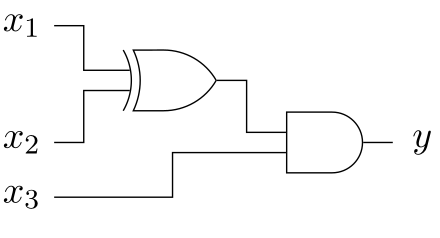
\includegraphics[width=300px]{images/gates38.3.png}\\
						$(x_1\oplus x_2)\land x_3$\\
						\begin{table}[h!]
\begin{tabular}{|l|l|l|l|l|}
\hline
$x_1$ & $x_2$ & $x_3$ & $x_1\oplus x_2$ & $x_3\land( x_1\oplus x_2)$ \\ \hline
1    & 1    & 1    & 0                              & 0                                                        \\ \hline
1    & 1    & 0    & 0                              & 0                                                         \\ \hline
1    & 0    & 1    & 1                              & 1                                                         \\ \hline
1    & 0    & 0    & 1                              & 0                                                         \\ \hline
0    & 1    & 1    & 1                              & 1                                                         \\ \hline
0    & 1    & 0    & 1                              & 0                                                         \\ \hline
0    & 0    & 1    & 0                              & 0                                                         \\ \hline
0    & 0    & 0    & 0                              & 0                                                         \\ \hline
\end{tabular}
\end{table}	
					\subsection{Lav et Boolsk udtryk med NOT, AND, OR og tre input variable, som har nedenstående tabel. Tegn også et tilsvarende kredsløb med tre inputs.}
						\begin{table}[h!]
						\begin{tabular}{|l|l|l|l|}
						\hline
						x\_1 & x\_2 & x\_3 & y \\ \hline
						0    & 0    & 0    & 0 \\ \hline
						0    & 0    & 1    & 0 \\ \hline
						0    & 1    & 0    & 1 \\ \hline
						0    & 1    & 1    & 0 \\ \hline
						1    & 0    & 0    & 1 \\ \hline
						1    & 0    & 1    & 0 \\ \hline
						1    & 1    & 0    & 0 \\ \hline
						1    & 1    & 1    & 1 \\ \hline
						\end{tabular}
						\end{table}
						$(\neg x_1\land x_2\land x_3)\lor ( x_1\land\neg x_2\land\neg x_3)\lor ( x_1\land x_2\land x_3)$
					\subsection{Vis hvordan man kan lave en OR-gate ved hjælp af AND-gates og
NOT-gates.(Til forelæsningen blev det vist, at alle boolske funktioner kan implementeres med AND-, OR-, og NOT-gates. Opgaven her viser, at AND- og NOT-gates er nok.)}
						$\neg(\neg x_1 \land \neg x_2)\rightarrow x_1\lor x_1$\\
						\subsection{Vis hvordan man kan lave en NOT-gate ved hjælp af en NAND-gate. Vis derefter hvordan man kan lave en AND-gate ved hjælp af NAND-gates. (Sammen med opgaven ovenfor viser dette, at NAND-gates er nok til at implementere alle boolske funktioner.)}
							$x_1\neg\land x_1\rightarrow \neg x_1$\\
							$(x_1\neg\land x_1)\neg\land(x_2\neg\land x_2)\rightarrow x_1\land x_2$\\
					\subsection{[Repetition fra forelæsningen.] Opskriv den korrekte tabel for funktionen Resultat(x1 ,x2 ,x3 ) fra slides om gates.}
						
						\begin{table}[h!]
						\begin{tabular}{|l|l|l|l|}
						\hline	
						$x_1$  & $x_2$  & $x_3$  & y \\ \hline
						0    & 0    & 0    & 0 \\ \hline
						0    & 0    & 1    & 1 \\ \hline
						0    & 1    & 0    & 1 \\ \hline
						0    & 1    & 1    & 0 \\ \hline
						1    & 0    & 0    & 1 \\ \hline
						1    & 0    & 1    & 0 \\ \hline
						1    & 1    & 0    & 0 \\ \hline
						1    & 1    & 1    & 1 \\ \hline
						\end{tabular}
						\end{table}
						
					\subsection{Opskriv tabellen for nedenstående kredsløb. Hvilken enkelt-gate svarerdet til?}
						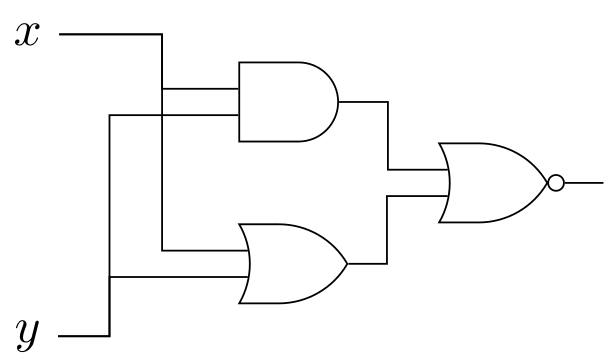
\includegraphics[width=300px]{images/38.1.1.png}
						\begin{table}[h!]
						\begin{tabular}{|l|l|l|}
						\hline
						x & y & output \\ \hline
						1 & 0 & 0      \\ \hline
						0 & 0 & 1      \\ \hline
						1 & 1 & 0      \\ \hline
						0 & 1 & 0      \\ \hline
						\end{tabular}
						\end{table}
						nand gate
					\subsection{Hvad er output af kredsløbet nedenfor?}
						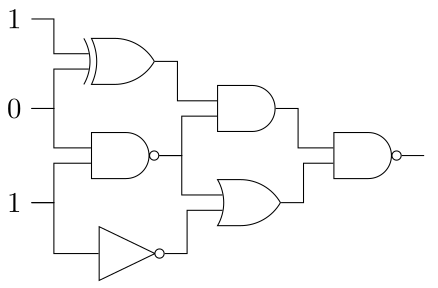
\includegraphics[width=300px]{images/38.1.2.png}\\
						1 1 1\\
						0 1 | 0\\
						1 0 1
					\subsection{Opskriv et Boolsk udtryk som svarer til samme kredsløb. Opskriv hele tabellen for kredsløbet.}
						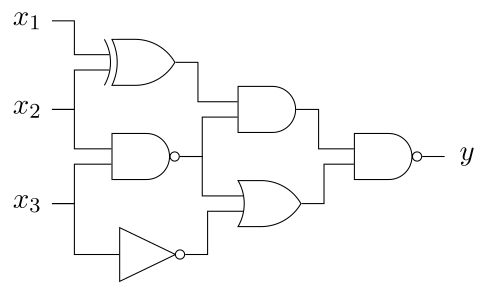
\includegraphics[width=300px]{images/38.1.3.png}\\
						$\neg(((x_1\oplus x_2) \land \neg(x_2\land x_3))\land(\neg(x_2\land x_3)\lor \neg x_3))$

						\begin{table}[h!]
						\begin{tabular}{|l|l|l|l|}
						\hline	
						$x_1$  & $x_2$  & $x_3$  & y \\ \hline
						0    & 0    & 0    & 1 \\ \hline
						0    & 0    & 1    & 1 \\ \hline
						0    & 1    & 0    & 0 \\ \hline
						0    & 1    & 1    & 1 \\ \hline
						1    & 0    & 0    & 0 \\ \hline
						1    & 0    & 1    & 1 \\ \hline
						1    & 1    & 0    & 1 \\ \hline
						1    & 1    & 1    & 1 \\ \hline
						\end{tabular}
						\end{table}
					\subsection{Lav et Boolsk udtryk med NOT, AND, OR og tre input variable, som har nedenstående tabel. Tegn også et tilsvarende kredsløb med tre inputs.}
						\begin{table}[h!]
						\begin{tabular}{|l|l|l|l|}
						\hline	
						$x_1$  & $x_2$  & $x_3$  & y \\ \hline
						0    & 0    & 0    & 1 \\ \hline
						0    & 0    & 1    & 1 \\ \hline
						0    & 1    & 0    & 0 \\ \hline
						0    & 1    & 1    & 0 \\ \hline
						1    & 0    & 0    & 1 \\ \hline
						1    & 0    & 1    & 0 \\ \hline
						1    & 1    & 0    & 1 \\ \hline
						1    & 1    & 1    & 0 \\ \hline
						\end{tabular}
						\end{table}
						$ (\neg x_1 \land \neg x_2 \land \neg x_3) \lor (\neg x_1 \land \neg x_2 \land x_3) \lor (x_1 \land \neg x_2 \land \neg x_3) \lor (x_1 \land x_2 \land \neg x_3)$\\
						$(\neg x_1 \land \neg x_2)\lor (x_1\land \neg x_3)$
				\subsection{[Repetition fra forelæsningen.] Opskriv den korrekte tabel for funktionen Mente(x1,x2,x3) fra slides om gates.}
					\begin{table}[h!]
						\begin{tabular}{|l|l|l|l|}
						\hline	
						$x_1$  & $x_2$  & $x_3$  & y \\ \hline
						0    & 0    & 0    & 0 \\ \hline
						0    & 0    & 1    & 0 \\ \hline
						0    & 1    & 0    & 0 \\ \hline
						0    & 1    & 1    & 1 \\ \hline
						1    & 0    & 0    & 0 \\ \hline
						1    & 0    & 1    & 1 \\ \hline
						1    & 1    & 0    & 1 \\ \hline
						1    & 1    & 1    & 1 \\ \hline
						\end{tabular}
					\end{table}|
				\subsection{Repetér hvordan I lærte i folkeskolen at gange flercifrede tal i 10-talsystemet sammen (på papir, uden lommeregner). Lav f.eks. regnestykkerne $123\cdot 432$ og $321\cdot 765$. Overvej hvorfor det virker (husk definitionen af 10-talsystemet, se evt. slides). Brug derefter samme princip til at lave en gangemetode i 2-talsystemet. Lav f.eks. regnestykkerne $111_2 \cdot 101_2$ og $10110_2 \cdot 11110_2$ på denne måde. Check at du har regnet rigtigt ved at konverterer de fire tal samt de to resultater fra 2-talsystemet til 10-talsystemet og derefter gange sammen på lommeregner der. Forklar metoden, og argumentet for at den fungerer, klarest muligt for hinanden}
					$101_2\cdot 111_2$
					\begin{tabular}{ccccccc}
					  &  &  &  & & 1 & 0 $1_2$ \\
					 &  & & & 1 & 0 & 1 $0_2$\\
					+ &  & & 1 & 0 & 1 & 0 $0_2$\\
					\hline
					 &  & 1 & 0 & 0 & 0 &1  $1_2$ \\
					\end{tabular}\
				\subsection{Hvad er den hexadecimale notation for kommandoerne til at gøre følgende (husk at numre på registre og RAM celler angives hexadecimalt)}
					\subsubsection{Kopiere indholdet af register C til RAM celle 0A.}
						$3C0A$	
					\subsubsection{Lægge bitmønstret 10110011 ind i register 2.}
						$22b3$
					\subsubsection{Addere register 3 og 4, og lægge resultatet i register 5.}
						$6534$
					\subsubsection{Lave bit-wise XOR af register B og C.}
						$9BBC$ XOR resultatet ligges i $B$
					\subsubsection{Hoppe til instruktionen i RAM celle 14 hvis indholdet i register C er større $(>)$ end indholdet i register 0.}
						$DC14$
				\subsection{Forklar følgende kode}
					\begin{lstlisting}
						1110
						1212
						5112
						1214
						5112
						3118
						C000
					\end{lstlisting}
					Koden tager data fra celle 10 og 12 og addere dem sammen i register 1 og nulstilelr reigster 2.
				\subsection{Lav et program som læser to heltal fra RAM cellerne 10 og 12, finder deres sum, og skriver resultatet i RAM celle 14. [Hint: det er en let forandring af det første eksempelprogram.]}
					Her skal $1214$ ændres til $3114$
					\subsection{Lav et program som læser et heltal k fra RAM celle 18 og som skriver summen $1 + 2 + 3 + . . . + (k - 1)$ i RAM celle E1. [Hint: det er en let forandring af det andet eksempelprogram.] Da man med 8 bits heltal i two’s complement kun kan repræsentere heltal op til 127, skal vi have $k \leq 16$ for at kunne repræsentere resultatet.}
						\begin{lstlisting}
							2000
						2101
						1518
						301E
						5404
						5001
						D506
						C000
						0000
						0000
						0000
						0000
						0800
						0000
						0000
						0700
						\end{lstlisting}
					\subsection{Lav et program som læser to heltal fra RAM celle 16 og 18, og som skriver det største af dem i celle 14.}
						\begin{lstlisting}
							1016
							1118
							D10A
							3014
							C000
							3114
							C000
							0000
							0000
							0000
							0500
							0500
							0400
						\end{lstlisting}
					\subsection{Lav et program som læser et heltal k fra RAM celle 20 og som skriver bitmønsteret 11111111 (hexadecimalt: FF) i RAM celle 22 hvis k er forskellig fra 0, og skriver bitmønsteret 01010101 (hexadecimalt: 55) i RAM celle 22 hvis k er lig 0}
						\begin{lstlisting}
							100c
							1120
							B108
							3222
							C000
							3355
							C000
							0100
						\end{lstlisting}

					\subsection{Lav et program som læser et bitmønster fra RAM celle 10, laver de første fire bits om til 0’er, og skriver svaret i RAM celle 12. Hint: det kan gøres med bit-wise AND med et bestemt bitmønster (hvilket?).}
						\begin{lstlisting}
							1010
							110E
							8010
							3012
							3355
							C000
							0000
							0F00
							FF00
						\end{lstlisting}
					\subsection{Lav et program som læser to bitmønster x og y fra RAM cellerne 20 og 22, laver et nyt bitmønster, som består af de første fire bits fra x efterfulgt at de sidste fire bits fra y, og skriver svaret i RAM celle 22. Hint: brug ideen fra sidste opgave to gange, samt bit-wise OR}
						\begin{lstlisting}
							1020
							1122
							1216
							1318
							8003
							8112
							7010
							3022
							C000
							0000
							0000
							0F00
							F000
							0000
							0000
							0000
							C800
							9900
						\end{lstlisting}
					\subsection{Lav et program som læser to bitmønster x og y fra RAM cellerne 20 og 22, laver et nyt bitmønster, som består af de sidste fire bits fra y efterfulgt at de første fire bits fra x, og skriver svaret i RAM celle 22. Hint: brug ideen fra sidste opgave, samt cyklisk rotation af bits.}
						\begin{lstlisting}
							1020
							1122
							1216
							1318
							8003
							8112
							7010
							3022
							C000
							0000
							0000
							F000
							0F00
							0000
							0000
							0000
							C800
							9900
						\end{lstlisting}
				\section{Uge}
					\subsection{Løs opgaven fra sidste side i slides om CPUer og maskinkode, dvs. lav et program som tæller ned i stedet for op. Mere præcist, lav et program som efter tur skriver tallene 6, 5, 4, 3,. . . , 0 (dvs. indhold 06, 05, 04, 03,. . . , 00) i RAM celle 1E, hvis RAM celle 18 indeholder 07 til at starte med.}
						\begin{lstlisting}
							1018
							1118
							1216
							5002
							301E
							B40E
							D106
							C000
							0000
							0000
							0000
							FF00
							0700
						\end{lstlisting}
					\subsection{I opgave II.12 fra uge 36/37 blev beskrevet følgende alternative metode til at skifte fortegn på heltal repræsenteret i two’s complement:Invertér alle bits i tallet og læg derefter 1 til tallet. Implementer denne metode i et program. Mere præcist, lav et program som læser et heltal x (i two’s complement) fra RAM celle 20 og skriver tallet $-x$ (i two’s complement) i celle 22. [Hint: bits i x kan inverteres ved bitwise XOR af x med et bestemt bitmønster (hvilket?).]}
						\begin{lstlisting}
							1020
111E
2201
9001
3022
6020
C000
0000
0000
0000
0000
FF00
0700
0000
0000
FF00
0C00
F300

					\end{lstlisting}
				\subsection{Multiplikation}
					\begin{lstlisting}
						1134
						1236
						2701
						2300
						2800
						8571
						5777
						2A01
						3313
						A501
						2600
						B522
						5626
						500A
						D318
						5886
						533A
						4070
						B10A
						D10A
						C000
						0200
						0500
					\end{lstlisting}
		\setcounter{subsection}{0}
		\subsection{Er følgende en algoritme}
		\begin{lstlisting}
			i=0
			while i != 5
				i=i+2
		\end{lstlisting}
			Nej denn terminere ikke
		\subsection{Betragt listen $L=[1,2,3,4,5,6,...,20]$. I nedenst[ende spørgsmål tæller vi sammenligninger som involverer elementer i listen.}
			\subsubsection{Hvor mange sammenligninger foretages der med SequentialSearch($L$, 7)?}
				7
			\subsubsection{Hvor mange sammenligninger foretages der med BinarySearch($L$, 7)?}	
				3 - 10, 5, 7
			\subsubsection{Antag nu, at $L$ indeholder 10.000 elementer. Hvor mange sammenligninger foretager man i værste tilfælde med en sekventiel søgning i $L$?}
				10.000
			\subsubsection{Hvor mange sammenligninger foretager man i værste tilfælde med en binær søgning i $L$?}
				$\frac{\ln{n}}{\ln{2}}$\\
				$\frac{\ln{10000}}{\ln{2}}=14$
		\subsection{Udfyld de manglende felter (undtagen dem i øverste række) i tabellen
på side 11 i slides fra Lenes forelæsning}
			Mængden af operationer udført på en given tid med en givet O nationen.\\
			$10^9\frac{1}{\si{s}}\cdot 1\si{s}=\log_2(n)$\\
			$n=4.6\cdot 10^{300000000}$\\
			\begin{table}[h!]
			\begin{tabular}{|l|l|l|l|l|l|}
			\hline
			 		& 1ms 		& 1s 		& 1min 			& 1 day 			& 1 year \\\hline
			$\log_2 n$   & $10^{300,000}$ 	&      $4.6\cdot 10^{300000000}$   	&                   $\infty$		&                $\infty$   		&    $\infty$         \\\hline
			$n$               & $10^6$                & $10^9$ 	& $6\cdot 10^{10}$ 	& $9\cdot 10^{13}$ 	& $3\cdot 10^{16}$ \\\hline
			$n \log_2 n$ & $6\cdot 10^4$ 	&    $4\cdot 10^7$               &  $2\cdot 10^9$                                      & $2\cdot 10^{12} $	&   $6 \cdot 10^{14}$                                   \\\hline
			$n^2$  	& $10^3$                &     32000              &   250000   			           & $9\cdot 10^6$      	&    $2\cdot 10^8$                       \\\hline
			$n^3$           & $10^2$                & $10^3$ 	&               $4\cdot 10^3$ 		           & $4\cdot 10^4$      	&   $3\cdot 10^5$                                                  \\\hline
			$2^n$       	& 20                         & 30   	&             36              		&         46                          	& 55             \\                                    \hline
			\end{tabular}
			\end{table}
		\subsection{Hvilken af følgende udsagn er sande?}
			\subsubsection{$n\in O(n)$}
				True
			\subsubsection{$2n+5\in O(n)$}
				True
			\subsubsection{$\sqrt{n}-\log(n)\in O(n)$}
				True
			\subsubsection{$(\log(n))^2\in O(n\log n)$}
				True
			\subsubsection{$n^2 \in O(n)$}
				False
			\subsubsection{$n\in O(n^2)$}
				True
			\subsubsection{$n\log(n)\in O(n^2)$}
				True
			\subsubsection{$n\log(n)\in O(n)$}
				False
			\subsubsection{$3n^2+2n+1\in O(n^2)$}
				True
			\subsubsection{$3n^2+2n+1\in O(n)$}
				False
		\subsection{Angiv for hver af følgende algoritmer deres asymptotiske køretid i $O$-notation som funktion af $n$}
			\begin{center}
				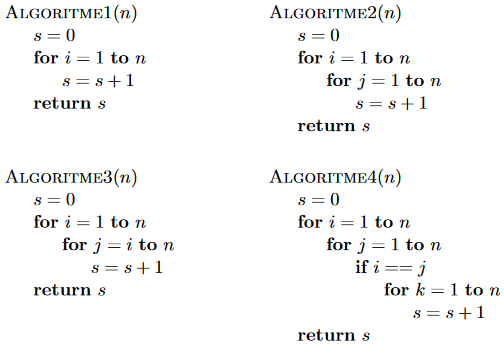
\includegraphics[width=250px]{images/40.5Algoritmer.png}
			\end{center}
			\subsubsection{Algoritme 1}
				$O(n)$
			\subsubsection{Algoritme 2}
				$O(n^2)$
			\subsubsection{Algoritme 3}
				$O(n^2)$
			\subsubsection{Algoritme 4}
				$O(n^2)$
		\subsection{Betragt følgende algoritme til at finde det mindste tal i lsiten $L$.}
			\begin{lstlisting}
Min(L)
n = L.length
min = L[1]
For i = 2 to n
	If L[i] < min
		min = L[i]
return min
			\end{lstlisting}
			\subsubsection{Hvad er algoritmens køretid}
				$O(n)$
			\subsubsection{Opskriv en løkke-invariant for algoritmen og bevis at den altid finder det mindste lement i $L$}
				$x\geq min$ for $n$
			\subsubsection{Omskriv algoritmen så den bruger en while-løkke i stedet for en for-løkke}
				\begin{lstlisting}
Min(L)
n = L.length
min = L[1]
i=2
while(i<=n)
	If L[i] < min
		min = L[i]
	i++
return min
			\end{lstlisting}
			\subsubsection{Bemærk at algoritmen er iterativ skriv en rekursiv version af algoritmen}
			\begin{lstlisting}
Min(L,i,min)
n = L.length
If i<=n
	If L[i] < min
		min = L[i]
	return Min(L,i+1,min)
return min
			\end{lstlisting}
		\setcounter{subsection}{0}
		\subsection{Hvilke af følgende udsagn er sande?}
			\subsubsection{$n\in O(n^3)$}
				True
			\subsubsection{$n^3\in O(n^2)$}
				False
			\subsubsection{$\log(n)\in O(n)$}
				True
			\subsubsection{$n\in O(n\log(n))$}
				True
			\subsubsection{$0.1n^2+n+10\in O(n)$}
				False
			\subsubsection{$0.1n^2+n+10\in O(n^2)$}
				True
			\subsubsection{$0.1n^2+n+10\in O(n^3)$}
				True
			\subsubsection{$n^2\log(n)\in O(n^2)$}
				False
		\subsection{Angiv for følgende algoritme dens asymptotiske køretid i $O$-notation som funktion af $n$}
			\begin{lstlisting}
s = 0
for i = 1 to n
	for j = i to n
		for k = i to j
			s = s + 1
return s
			\end{lstlisting}
			$O(n^3)$
		\subsection{Husk på algoritmerne til, ciffer for ciffer, at addere eller gange to tal i hånden}
			\subsubsection{Hvad er køretiden for at addere to tal med $n$ cifre hver? Hvad er den karakteristiske operation?}
				$O(n)$ Der sker en lille adition mellem hvert ciffer med de to tal og mende
			\subsubsection{Hvad er køretiden for at gange to tal med $n$ cifre hver? Hvad er den karakteristiske operation?}
				$O(n^2)	$
	\section{Uge}
		\subsection{Opskriv i pseudokode algoritmen Sequential Search ved hjælp af operationerne readNext(), isEndOfFile(), open() og close() fra interfacet sekventiel tilgang.}
			\begin{lstlisting}
file = open()
int i = 0;
while(!file.isEndOfFile())
		if(file.readNext() == search)
			return i;
		i++;
file.close()
return not found
			\end{lstlisting}
		\subsection{Opskriv i pseudokode algoritmen for merge af to lister ved hjælp af operationerne readNext(), isEndOfFile(), writeNext(data), open() og close() fra interfacet sekventiel tilgang.}
			\begin{lstlisting}
file1 = open()
file2 = open()
i1 = file1.readNext()
i2 = file2.readNext()
merge = []
while(!file1.isEndOfFile() && !file2.isEndOfFile())
	if (i1>i2)
		merge.push(i1)
		i1 = file1.readNext()
	else
		merge.push(i2)
		i2 = file2.readNext()
if (file1.isEndOfFile())
	while(!file1.isEndOfFile())
		merge.push(file1.readNext())
else
	while(!file2.isEndOfFile())
		merge.push(file2.readNext())
file1.close()
file2.close()
			\end{lstlisting}
		\subsection{I denne opgaver repræsenterer vi mængder som sorterede lister uden dubletter. For eksempel vil de to mængder $A = \{5, 3, 9, 8\}$ og $B =\{3, 2, 9, 10, 27\}$ være repræsenteret som disse sorterede lister: $$A = [3, 5, 8, 9]$$ $$B = [2, 3, 9, 10, 27]$$ Beskriv en algoritme til at beregne repræsentationen af forenings mængden $X\cup Y$ ud fra repræsentationen af to mængder $X$ og $Y$.}
			En algoritme ville foregå således.\\
			Tag første element i begge lister, hvis de ikke er lig med hinaden tages den laveste. Hvis de er lig med hinanden tages kun én og den anden fjernes. \\
			Dette udføres indtil en liste er tom hvorefter den anden ligges oven i.
		\subsection{Beskriv en algoritme til at flette (merge) indholdet af tre sorterede lister $A$, $B$ og $C$ sammen til en sorteret liste $D$. Hvad er køretiden for din algoritme?}
		Denne algoritme er den samme som mergesort. Dermed er køretiden $O(n)$
		\subsection{Givet en algoritme til at flette indholdet af tre sorterede lister $A$, $B$ og $C$ sammen til én sorteret liste $D$ (dvs. givet en løsning til opgave 4), beskriv en variant af Mergesort baseret på denne. Hvad er køretiden for din algoritme?}
			For den første mergesort vil der være 2 lister med 1 element, som begge er sorteret\\
			I denne mergesort vil det først element blive placeret først.\\
			Ved denne næste merge vil det mindste element igen tages først og dermed vil det nye element placeres korrekt i listen.
		\subsection{Hvis en hashfunktion $h$ er givet ved $h(x) = x \% 11$, på hvilke pladser i tabellen ender tallene 25, 75, 125, 175?}
			$25 \rightarrow 3$\\
			$75 \rightarrow 9$\\
			$125 \rightarrow 4$\\
			$175 \rightarrow 10$
		\subsection{Hvis en hashfunktion h er givet ved $h(x) = x \% 11$, hvor mange pladser i hashtabellen har mere end ét element, når der indsættes elementerne 34, 65, 122 og 155?}
			$34 \rightarrow 1$\\
			$65 \rightarrow 10$\\
			$122 \rightarrow 1$\\
			$155 \rightarrow 1$\\
			Dermed 3 på 1
		\subsection{Beregn med lommeregner svaret på følgende: Hvis 3 elementer indsættes tilfældigt i et array med 7 pladser, hvad er sandsynligheden for, at der ikke er to elementer som ender på samme plads?}
			\begin{align*}
				s_n=s_{n-1}\cdot \frac{7-(n-1)}{7}\\
				s_0=1\cdot \frac{7-0}{7}=1\\
				s_1=1\cdot \frac{7-1}{7}=0.86\\
				s_2=0.86\cdot \frac{7-2}{7}=0.61\\
				s_3=0.61\cdot \frac{7-3}{7}=0.35
			\end{align*}
		\subsection{Beregn med lommeregner følgende svaret på følgende: Hvis 5 elementer indsættes tilfældigt i et array med 12 pladser, hvad er sandsynligheden for, at der ikke er to elementer som ender på samme plads?}
			\begin{align*}
				s_0=1\\
				s_1=1\cdot \frac{12-1}{12}=0.92\\
				s_2=0.92\cdot \frac{10}{12}=0.77\\
				s_3=0.77\cdot \frac{9}{12}=0.58\\
				s_4=0.58\cdot \frac{8}{12}=0.39\\
				s_5=0.39\cdot \frac{7}{12}=0.23
			\end{align*}
		\setcounter{subsection}{0}
		\subsection{Hvis en hashfunktion $h$ er givet ved $h(x) = x \% 17$, på hvilke pladser i tabellen ender tallene 22, 72, 122, 172?}
			$22 \rightarrow 5$\\
			$72 \rightarrow 4$\\
			$122 \rightarrow 3$\\
			$172 \rightarrow 2$
		\subsection{Hvis en hashfunktion $h$ er givet ved $h(x) = x \% 17$, hvor mange pladser i hashtabellen har mere end ét element, når der indsættes elementerne 40, 74, 101 og 159?}
			$40 \rightarrow 6$\\
			$74 \rightarrow 6$\\
			$101 \rightarrow 16$\\
			$159 \rightarrow 6$\\
			Dermed 3 på plads 6
		\subsection{Lav et Java-program med input $n$ og $k$ der for situationen hvor $n$ elementer indsættes tilfældigt i et array med k pladser finder sandsynligheden for, at der ikke er to elementer som ender på samme plads.}
			Kan findes i mappen  collisionChance
		\subsection{Hvis 1000 elementer indsættes tilfældigt i et array med 1.000.000 pladser, hvad er sandsynligheden for, at der ikke er to elementer som ende på samme plads?}
			61\% chance
		\subsection{Hvis $n$ elementer indsættes tilfældigt i et array med 1.000.000 pladser, hvor stor skal $n$ være for at sandsynligheden for, at der ikke er to elementer som ender på samme plads, bliver mindre end $\frac{1}{2}$}
			1177 fundet via programmet.
		\subsection{[Udfordrende] Beskriv en algoritme, der som input tager et tal $K$ og to sorterede lister $X$ og $Y$ , hver med $n$ tal, og finder ud af, om der findes et par at tal $x \in X$ og $y \in Y$ for hvilke $x + y = K$. Din algoritme skal køre i tid $O(n)$. Du skal argumentere for køretiden og for korrektheden af svaret.}
			\begin{lstlisting}
additionElement(K,L1,L2):
int j = L2.length;
int i = 0;
while(i<L1.length && j >=0)
	if (L1[i]+L2[j]==K)
		return True;
	else if (L1[i]+L2[j]>K)
		j--;
	else
		i++;
return False;
			\end{lstlisting}
			Med kun 1 loop vil den værste køretid være $O(n)$. Korrektheden kan findes i at, i tilfælde at additionen blvier for stor vil den rykke således at værdien vil blive mindre og bliver det større rykker den således listens værdier bliver mindre. Jeg tror dog at der er en fejl hvor det kan lade sig gøre at misse en værdi...
	\section{Uge}
		\subsection{Exerise. $k$-Neares Neighbors: Prediction}
			What would the value of $x=8$ be using 5-nearest neightbors and what form of learning is this exercise.\\
			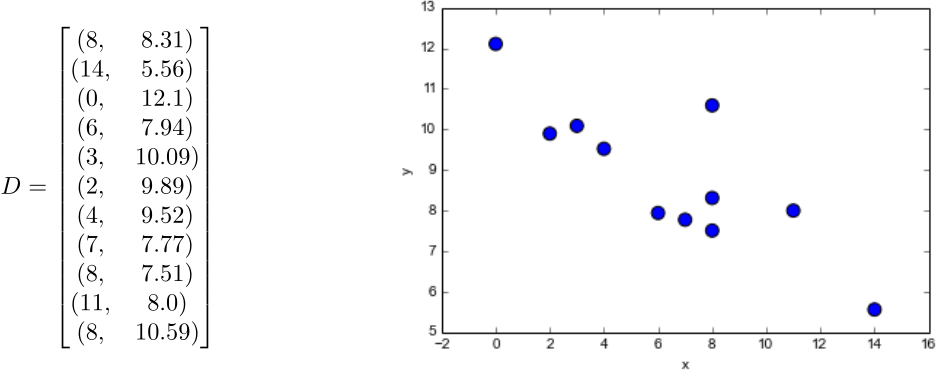
\includegraphics[width=\linewidth]{images/41,1.png}\\
			$\hat{y}(x)=\frac{1}{k}\sum\limits_{i|x_i\in N_k(x)}y_i=\frac{1}{5}(8.31+7.94+7.77+7.51+10.59)=8.424$\\
			Supervised learning, regression. Supervised due to a correct value and regression due to the  corresponding value being a value not being binary.
		\subsection{Exercise. $k$-Nearest Neighbors: Prediction}
			Predict $\vec{x}=(5,10)$ with 5 nearest neighburs and determine the type og learning.\\
			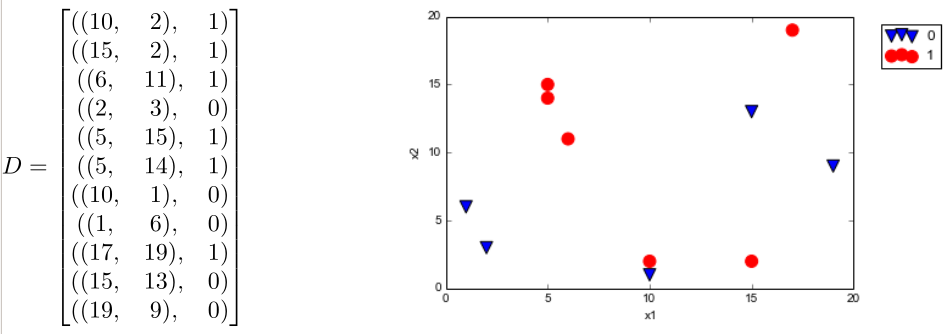
\includegraphics[width=\linewidth]{images/41,2.png}\\
			Here the difference was found and totalle between the two points and the best was chosen.\\
			$\frac{1+1+1+0+0}{5}=1$\\
			Supervised learning classification.
		\subsection{Exercise. Linear Regression: Prediction}
			Find the value of $x=8$ now with a linear regression model $g(x)=-0.37x+11.2$\\
			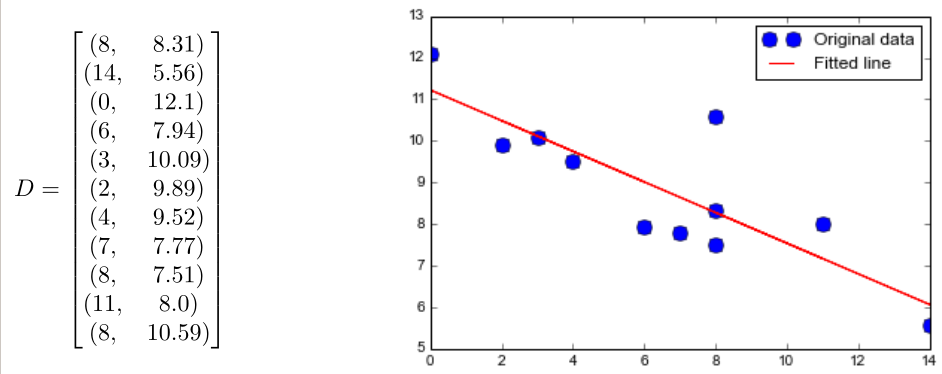
\includegraphics[width=\linewidth]{images/41,3.png}\\
			$g(8)=-0.37\cdot 8+11.2=8.24$\\
		\subsection{Exercise. Linear Regression: Training}
			Calculate the linear regression and the lost from the lose function.\\
			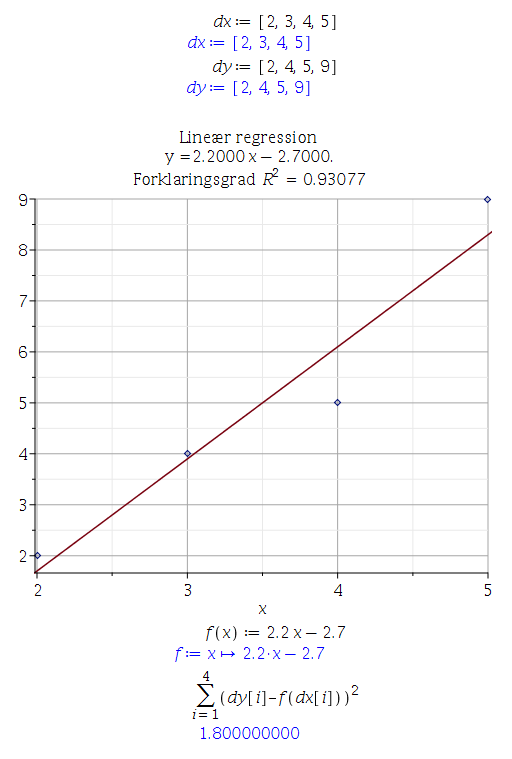
\includegraphics[width=300px]{images/41,4.png}
		\subsection{Exercise. Logical Functions and Perceptrons}
			Create truth table for the following perceptron gates
			\subsubsection{OR gate}
				Here the $W_0=0.5, W_1=1, W_2=1$\\
				\begin{table}[h!]
				\begin{tabular}{|l|l|l|l|}
				\hline
				$input_1$ & $input_2$ & sum & output \\ \hline
				1     & 1     & 2   & 1      \\ \hline
				1     & 0     & 1   & 1      \\ \hline
				0     & 1     & 1   & 1      \\ \hline
				0     & 0     & 0   & 0      \\ \hline
				\end{tabular}
				\end{table}		
			\subsubsection{NOT gate}
				Here the $W_0=-0.5, W_1=-1$\\
				\begin{table}[h!]
				\begin{tabular}{|l|l|l|}
				\hline
				$inut_1$ & sum & output \\ \hline
				1     & -1   & 0      \\ \hline
				0     & 0   & 1      \\ \hline
				\end{tabular}
				\end{table}	
			\subsubsection{Create NAND gate}
				$W_0=-1.5, W_1=-1, W_2=-1$
		\subsection{Exercise. Multilayer Perceptrons}
			Determinde the truth table for the following figure.\\
			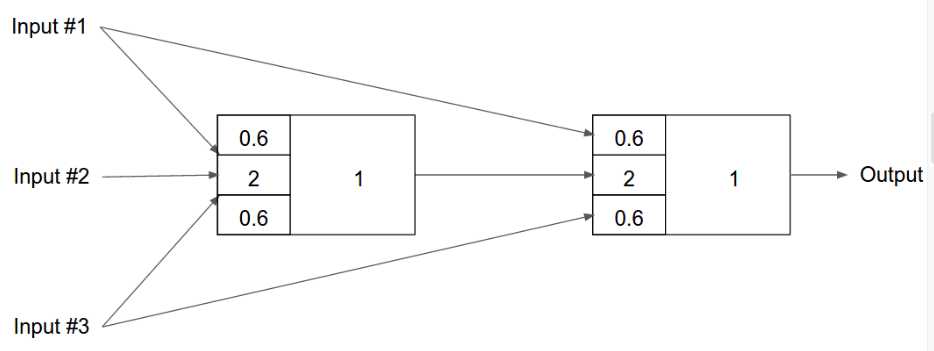
\includegraphics[width=\linewidth]{images/41,6.png}\\
			\begin{table}[]
			\begin{tabular}{|l|l|l|l|l|}
			\hline
			$input_1$ & $input_2$ & $input_3$ & Perceptron1 & Perceptron2 \\ \hline
			1         & 1         & 1         & 1           & 1           \\ \hline
			1         & 0         & 1         & 1           & 1           \\ \hline
			0         & 1         & 1         & 1           & 1           \\ \hline
			0         & 0         & 1         & 0           & 0           \\ \hline
			1         & 1         & 0         & 1           & 1           \\ \hline
			1         & 0         & 0         & 0           & 0           \\ \hline
			0         & 1         & 0         & 1           & 1           \\ \hline
			0         & 0         & 0         & 0           & 0           \\ \hline
			\end{tabular}
			\end{table}
		\subsection{Exercise. Single Layer Neural Networks: Prediction}
			The following exercises is based on the following perceptron which was trained in the data from 2 exercise.\\
			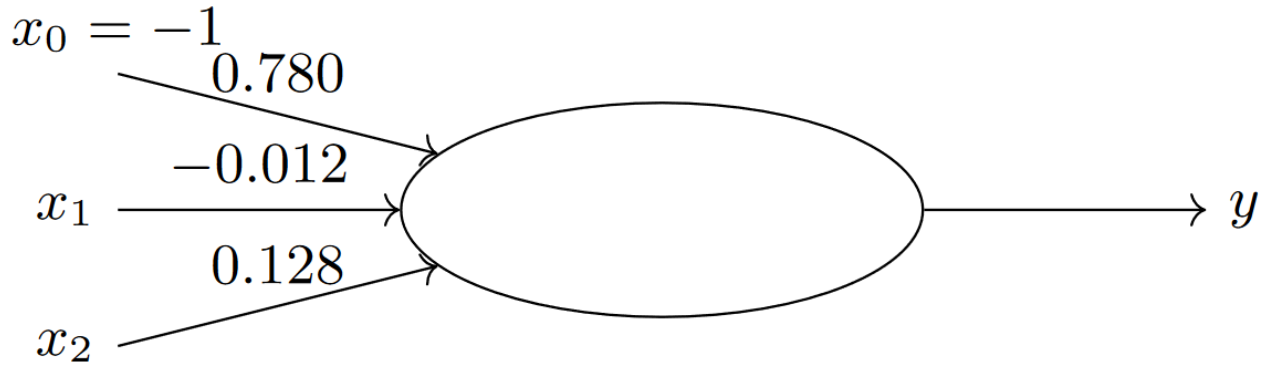
\includegraphics[width=\linewidth]{images/41,7.png}
			\subsubsection{Calculate output with $\vec{x}=(5,10)$ using step function}
				$-0.012\cdot 5 + 0.128\cdot 10-1\cdot 0.78=0.440$\\
				Since the result is above zero it will return 1.
			\subsubsection{Calculate output with $\vec{x}=(5,10)$ using sigmoid function}
				$\frac{1}{1+e^{-0.44}}=0.6$\\
				The answer is above 0.5 therefore it returns 1\\
			\subsubsection{Will the two functions always result in the same result, which one is more correct?}
				\begin{figure}[h!]
					\centering
					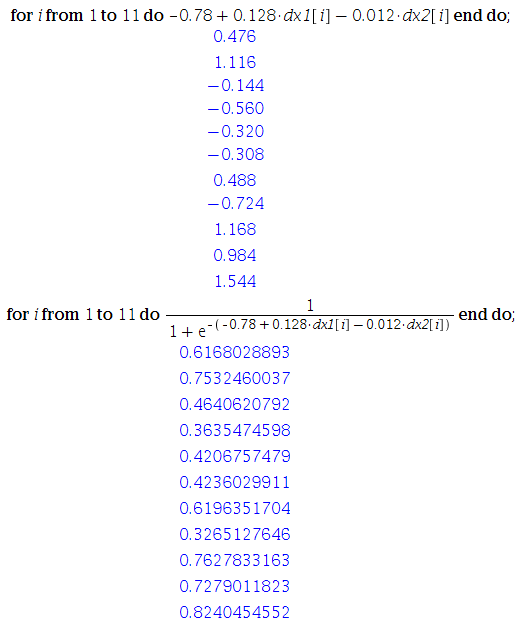
\includegraphics[width=300px]{images/41,7,3.png}
					\label{41.7.3}
					\caption{Beregning på punkter i D}
					\center
				\end{figure}
				As it can be seen both function will result in the asme result due to the sigmoid functions turning point being the at when the step function changes.\\
				As it can be seen the node is not perfect with 50\% being correct
			\subsubsection{Make a plot with the predictions and find a line}
				\begin{figure}[h!]
					\centering
					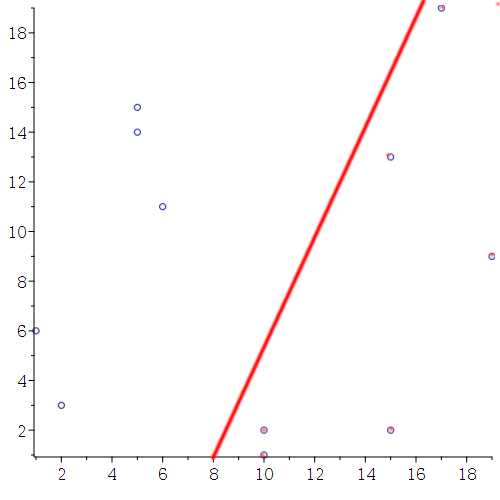
\includegraphics[width=300px]{images/41,7,4.png}
					\label{41,7,4}
					\caption{The ones classified is colores red}
				\end{figure}
		\subsection{Exercise. Expressivness of a single layer perceptron}
			A single layer perceptron will not be able to express a XOR gate
		\setcounter{subsection}{0}
		\subsection{Exercise. $k$'Nearest Neighbors: Prediction}
			Find $x=12$ using 3 nearest neighbors, on the folllowing data.\\
			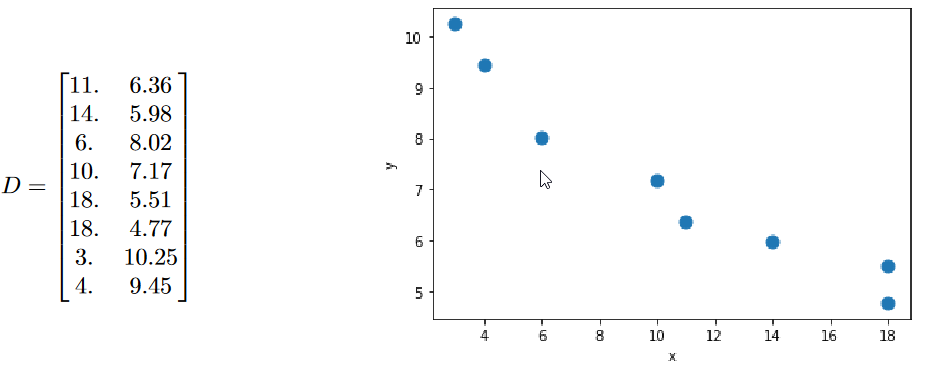
\includegraphics[width=\linewidth]{images/41,1,1.png}\\
			$\frac{7.17+6.36+5.98}{3}=6.50$\\
			This is a supervised learning regression.
		\subsection{Exercise. $k$-Nearest Neighbors: Prediction}
			Find $\vec{x}=(14,8)$ using 3 nearest neighbors, on the folllowing data.\\
			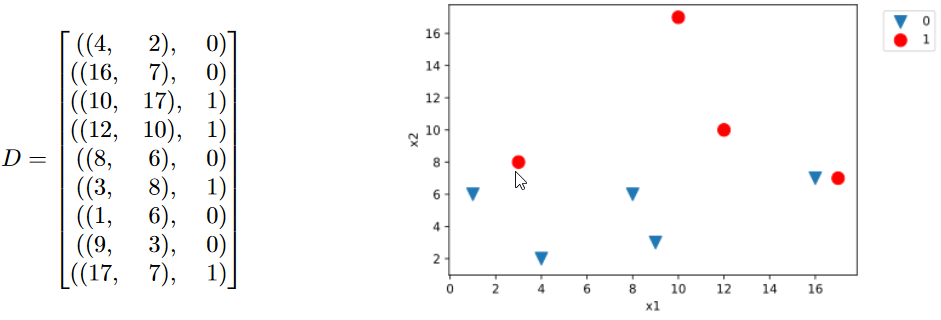
\includegraphics[width=\linewidth]{images/41,1,2.png}\\
			$1+0+1=2$ output 1\\
			Supervisedclassification
		\subsection{Exercise. Linear Regression: Training}
			Calculate the linear regression and the lost.
			\begin{align*}D=
			\left[\begin{array}{cc}
			    5&44\\
			    16&16\\
			    13&20\\
			    19&3\\
			    9&29
			\end{array}\right]
			\end{align*}\\
			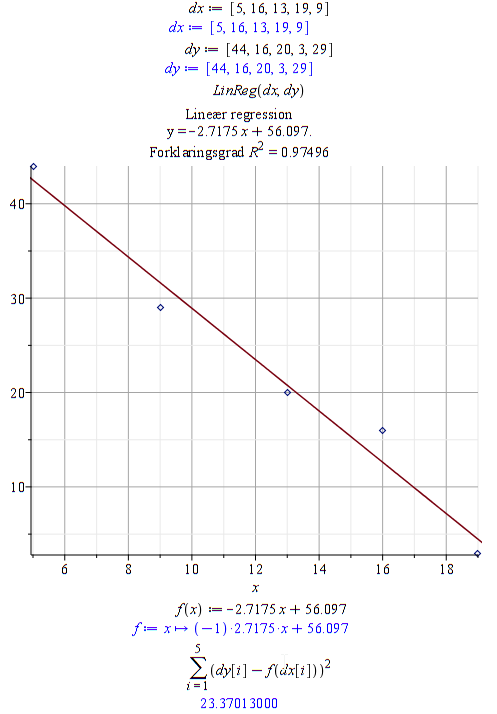
\includegraphics[width=300px]{images/41,1,3.png}
		\subsection{Exercise. Feed-Forward Neural Network: Single Layer Perceptron}
			Determine the parameters of a single p erceptron (that is, a neuron with step function) that implements the majority function: for n binary inputs the function outputs a 1 only if more than half of its inputs are 1.\\
			It will simply be a weight of 1 except the bias $w_0=\lfloor n \rfloor$
		\subsection{Exercise. Single Layer Perceptrons}
			Make the following neural network into a perceptron.\\
			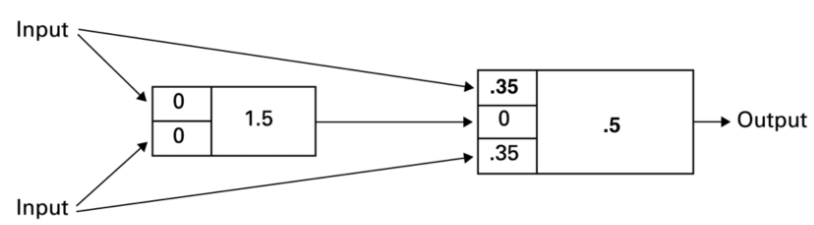
\includegraphics[width=300px]{images/41,1,5.png}\\
			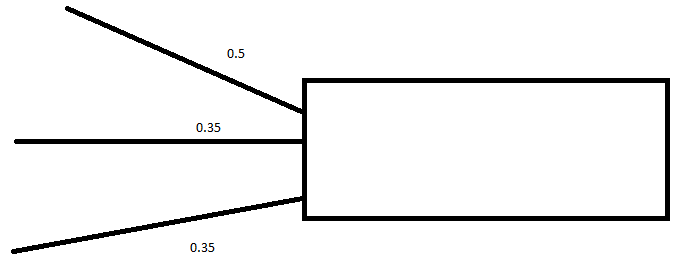
\includegraphics[width=300px]{images/41,1,5,1.png}
		\subsection{Exercis. Logical Functions and Neural Networks}
			We have to convert the following circuit with perceptrons from exercis 5. Just imagine it.\\
			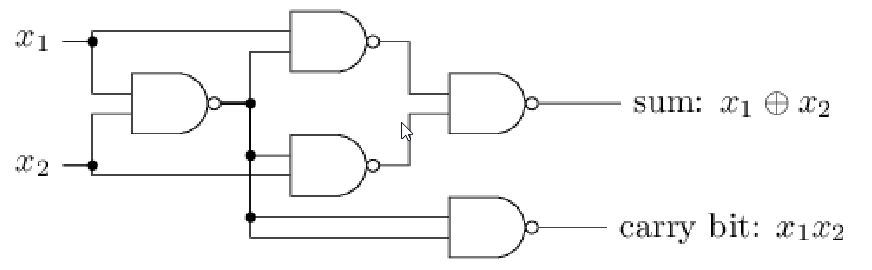
\includegraphics[width=300px]{images/41,1,6.png}
	\setcounter{section}{42}
	\section{uge}
		\subsection{Beregn følgende}
			\subsubsection{$L_3$-normen af $\vec{v}=(-2,5)$.}
				$(-2.5^3+5^3)^{1/3}=4.78$
			\subsubsection{$L_7$-normen af $\vec{v}=(4.5,-3.2)$.}
				$(4.5^7-3.2^7)^{1/7}=4.38$
			\subsubsection{$L_1$-normen af $\vec{v}=(5,9)$.}
				$(5^1+9^1)^{1/1}=14$
			\subsubsection{$L_{1.5}$-normen af $\vec{v}=(2,3)$.}
				$(2^{1.5}+3^{1.5})^{1/1.5}=4.01$
			\subsubsection{$L_\infty$-normen af $\vec{v}=(4.5,-3.2)$.}
			$(4.5^\infty -3.2^\infty )^{1/\infty}=max(4.5,-3.2)=4.5$
		\subsection{For $\vec{p}=(1,2,3)$ og $\vec{q}=(0,5,-2)$ beregn følgende:}
			\subsubsection{Afstanden $\text{dist}_2(\vec{p},\vec{q})$.}
				$(|1-0|^2+|2-5|^2+|3+2|^2)^{1/2}=5.92$
			\subsubsection{Afstanden $\text{dist}_3(\vec{p},\vec{q})$.}
				$(|1-0|^3+|2-5|^3+|3+2|^3)^{1/3}=5.35$
			\subsubsection{Afstanden $\text{dist}_1(\vec{p},\vec{q})$.}
				$(|1-0|^2+|2-5|^2+|3+2|^2)^{1/2}=35$
			\subsubsection{Afstanden $\text{dist}_\infty(\vec{p},\vec{q})$.}
			$(|1-0|^\infty+|2-5|^\infty+|3+2|^\infty)^{1/\infty}=max(1,3,5)=5$
		\subsection{Forklar figuren mudt på side 18 i Melih Kandemirs slides. Dvs. forkalr hvorfor mængden af alle punkter $\vec{q}$i en given afstand $r$ fra et punkt $\vec{q}$ (også kaldet "cirklen" om $\vec{q}$ med radius $r$) har en sådan facon, når afstanden er givet ved $\text{dis}_1$.}
		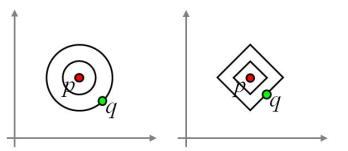
\includegraphics[width=300px]{images/43,2.png}
			Det komemr af at formen er ens med definitionen af en cirkel nemlig $(x-x_c)^2+(y-y_c)^2=r^2$ hvor det ene punkt er centrum for cirklen.
		\setcounter{subsection}{2}
		\subsection{Forklar også figuren til højre på samme side}
			En måde at se det på er, at afstanden vil her være hypotenusen i en retvinklet trekant. Dermed ved vinklerne bliver 0, 90, 270 og 360, vi ldet to kateter blot bliver summeret og de andre sted vil det være hypotenusen som er afstanden.
		\setcounter{subsection}{2}
		\subsection{Forsøg også at forklare, hvorfor $L_{\infty}$ er et godt navn for max-normen, når man sammenligner med definitionen af $L_p$}
			Da potensen og kvadratroden er så stor vil det betyde at desto højere tallet er vil det have markant mere effekt og derfor tages blot det højeste tal.
		\subsection{Consider the five picture given in Figure 1 each with 36 pixels.}
			\begin{figure}[h]
				\centering
				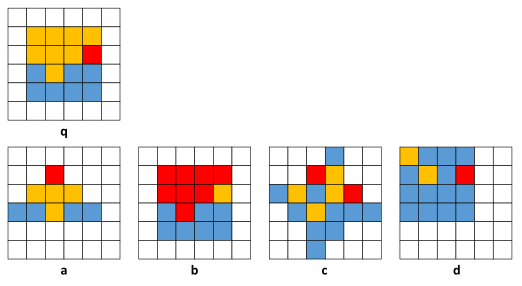
\includegraphics[width=\linewidth]{images/43,4.png}
				\label{pixelImages}
				\caption{$6\times 6$ pixel pictures}
			\end{figure}
			\subsubsection{Extract from each picture a color histogram with the bins $red, orange$, and $blue$ (the white pixels are ignored)}
			\begin{itemize}
				\item a - 1 4 4\\
				\item b - 8 1 7\\
				\item c - 2 4 10\\
				\item d - 1 2 13\\
				\item q - 1 8 7
			\end{itemize}
			\subsubsection{For each of the pictures $a$ to $d$, calculate their similarity to $q$ using Euclidean distance (i.e. using$\text{dist}_2$}
			\begin{itemize}
				\item a - $(|1-1|^2+|4-8|^2+|4-7|^2)^{0.5}=5$
				\item b - $(|8-1|^2+|1-8|^2+|7-7|^2)^{0.5}=9.9$
				\item c - $(|2-1|^2+|4-8|^2+|10-7|^2)^{0.5}=5.1$
				\item d - $(|1-1|^2+|2-8|^2+|13-7|^2)^{0.5}=8.49$
			\end{itemize}
			Therefore the closes approximation to $q$ is $a$
		\subsection{Repetér definitionen af en centroide for en cluster $C$ bestående af følgende tre punkter}
			$C=\{(2,3),(5,5),(4,1)\}$
			$(\frac{2+5+4}{3},\frac{3+5+1}{3})=(3.67,3)$
		\subsection{Check beregningen af de to centroder i figuren på side 32}
			blue $\{(1,5),(3,4),(10,1)\}$\\
			red $\{(7,7),(7,8),(6,8),(7,9)\}$
			red centroid $(\frac{1+3+10}{3},\frac{5+4+1}{3})=(4.67,3.33)$\\
			blue $(\frac{7+7+6+7}{4},\frac{7+8+8+9}{4})=(6.75,8)$
		\subsection{Consider the following data set (with 8 objects in $\mathbb{R}^2$) used in the lecture:}
			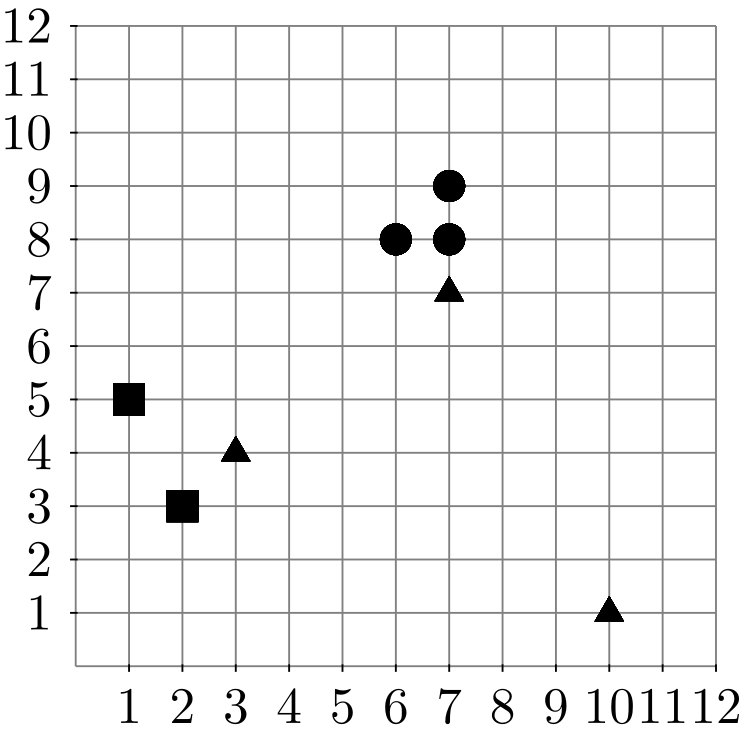
\includegraphics[width=300px]{images/43,7.png}
			\subsubsection{Compute a complete partitioning with $k=2,3,4,5$ using k means method}
				k = 2: (7.4,6.6), (2,4) - TD2 = 54.4\\
				k = 3: (10,1),(6.75,8),(2,4) - TD2 = 6.75\\
				k = 4: (10,1),(2.5,3.5),(1,5),(6.75,8) - TD2 = 3.75\\
				k = 5: (10,1),(6.5,7.5),(1.5,4),(3,4),(7,8.5) - TD2 = 4\\
				When the number of clusters became larger, many times it would cluster to a lower amount and clusters would just be at (0,0).
		\subsection{Repeter forskellen på Forgy-Lloyd og MacQueen udgaverne af k-means algoritmen, giver de to udgaver altid samme resultat.}
				Nej, ud fra punkternes tilfældige placering, giver det en variation ved begge algoritmer og dermed vil de aldrig med garanti give ens resultater. Derudover kan algoritmen også udføres på samme punkter og også give forskellige løsninger
	\section{Uge}
		\subsection{Exercise}
			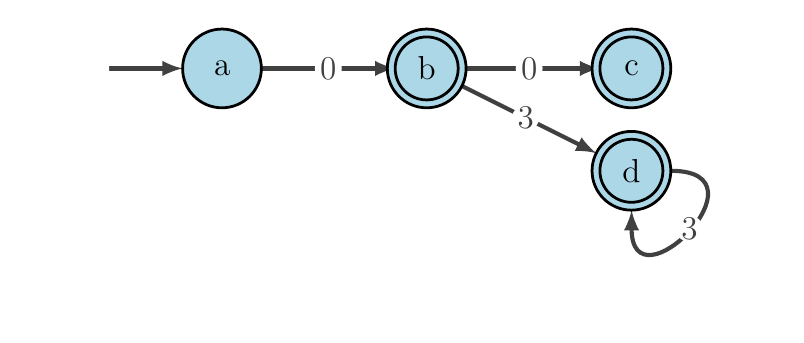
\begin{tikzpicture}[scale=1.3]
				\SetVertexStyle[MinSize=1\DefaultUnit,TextFont=\large]
				\SetEdgeStyle[TextFont=\large]
				\Vertex[x=0,style={color=white}]{Z}
				\Vertex[label=a,x=1.5]{A}
				\Vertex[x=5.5,y=-1]{D}
				\Vertex[label=b,x=3.5]{B}
				\Vertex[label=b,x=3.5,size=0.8]{B}
				\Vertex[label=c,x=5.5]{C}
				\Vertex[label=c,x=5.5, size=0.8]{C}
				\Vertex[label=d,x=5.5,y=-1, size=0.8]{O}
				\Edge[Direct](Z)(A)
				\Edge[Direct,label=0](A)(B)
				\Edge[Direct,label=0](B)(C)
				\Edge[Direct,label=3](B)(D)
				\Edge[Direct,label=3,loopposition=-45](D)(D)
			\end{tikzpicture}\\
			The following DFA will accept string starting with 0 followed by infite 3 or a zero or nothing.
		\subsection{Exercise}
			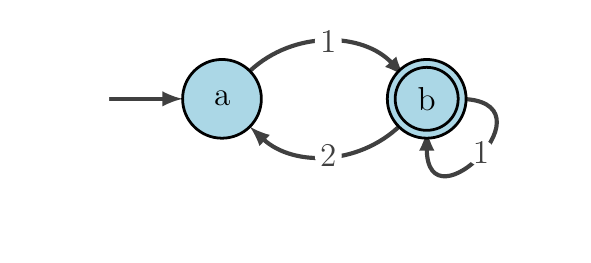
\begin{tikzpicture}[scale=1.3]
				\SetVertexStyle[MinSize=1\DefaultUnit,TextFont=\large]
				\SetEdgeStyle[TextFont=\large]
				\Vertex[x=0,style={color=white}]{Z}
				\Vertex[label=a,x=1.5]{A}
				\Vertex[label=b,x=3.5]{B}
				\Vertex[label=b,x=3.5,size=0.8]{B}
				\Edge[Direct](Z)(A)
				\Edge[Direct,label=1, bend=45](A)(B)
				\Edge[Direct,label=2, bend=45](B)(A)
				\Edge[Direct,label=1,loopposition=-45](B)(B)
			\end{tikzpicture}\\
			The following DFA will accept string startign with 1 followed by either any number of 1 or a 2 followed by any number of 1.
		\subsection{Exercis}
			Write a DFA which accepts strings containing a even number of zeros and odd number of 1\\
			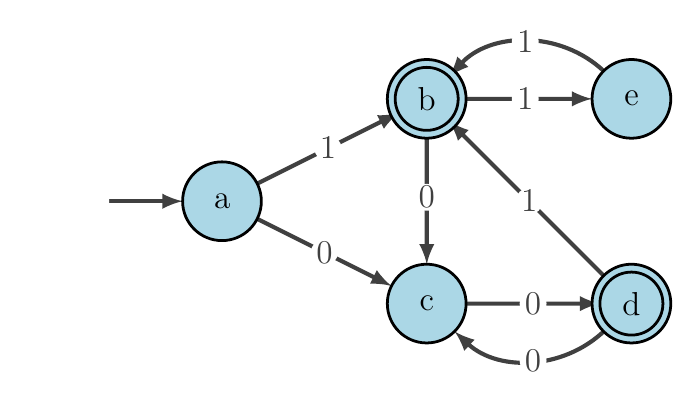
\begin{tikzpicture}[scale=1.3]
				\SetVertexStyle[MinSize=1\DefaultUnit,TextFont=\large]
				\SetEdgeStyle[TextFont=\large]
				\Vertex[x=0,style={color=white}]{Z}
				\Vertex[label=a,x=1.5]{A}
				\Vertex[label=b,x=3.5,y=1]{B}
				\Vertex[label=b,x=3.5,size=0.8,y=1]{B}
				\Vertex[label=c,x=3.5,y=-1]{C}
				\Vertex[label=d,x=5.5,y=-1]{D}
				\Vertex[label=d,x=5.5,y=-1,size=0.8]{D}
				\Vertex[label=e,x=5.5,y=1]{E}
				\Edge[Direct](Z)(A)
				\Edge[Direct,label=1](A)(B)
				\Edge[Direct,label=0](A)(C)
				\Edge[Direct,label=0](C)(D)
				\Edge[Direct,label=0,bend=45](D)(C)
				\Edge[Direct,label=1](B)(E)
				\Edge[Direct,label=0](B)(C)
				\Edge[Direct,label=1](D)(B)
				\Edge[Direct,label=1, bend=-45](E)(B)
			\end{tikzpicture}\\
		\subsection{Exercise}
			Make a DFA that accepts a string of 0 and 1 which contains 010\\
			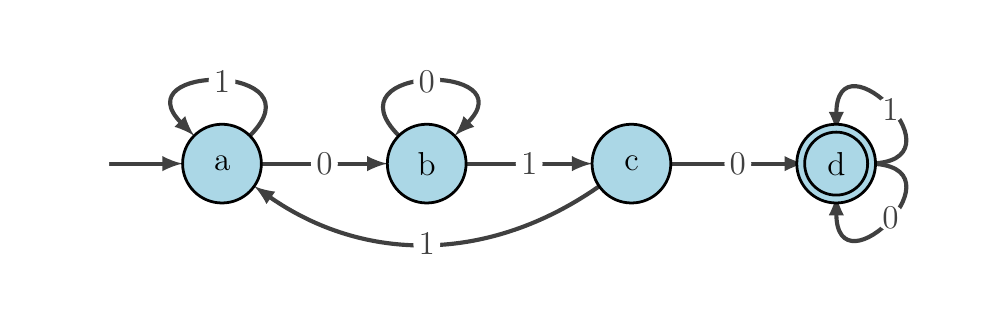
\begin{tikzpicture}[scale=1.3]
				\SetVertexStyle[MinSize=1\DefaultUnit,TextFont=\large]
				\SetEdgeStyle[TextFont=\large]
				\Vertex[x=0,style={color=white}]{Z}
				\Vertex[label=a,x=1.5]{A}
				\Vertex[label=b,x=3.5]{B}
				\Vertex[label=c,x=5.5]{C}
				\Vertex[label=d,x=7.5]{D}
				\Vertex[label=d,x=7.5,size=0.8]{D}
				\Edge[Direct](Z)(A)
				\Edge[Direct,label=0, bend=0](A)(B)
				\Edge[Direct,label=1](B)(C)
				\Edge[Direct,label=1,loopposition=90,loopshape=-90](A)(A)
				\Edge[Direct,label=0,loopposition=90,loopshape=90](B)(B)
				\Edge[Direct,label=0,bend=0](C)(D)
				\Edge[Direct,label=1,bend=35](C)(A)
				\Edge[Direct,label=1,loopposition=45,loopshape=-90](D)(D)
				\Edge[Direct,label=0,loopposition=-45,loopshape=90](D)(D)
			\end{tikzpicture}\\
		\subsection{Exercise}
			Define a DFA that recignises the following languageL Akk strings of 0s and 1s that contain at least two occurrences of 10 and an even number of 0s.
			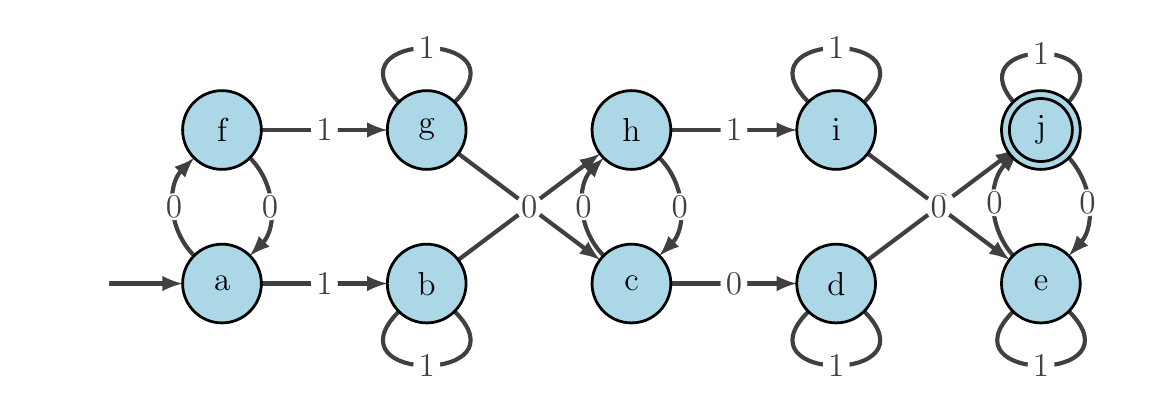
\begin{tikzpicture}[scale=1.3]
				\SetVertexStyle[MinSize=1\DefaultUnit,TextFont=\large]
				\SetEdgeStyle[TextFont=\large]
				\Vertex[x=0,style={color=white}]{Z}
				\Vertex[label=a,x=1.5]{A}
				\Vertex[label=b,x=3.5]{B}
				\Vertex[label=c,x=5.5]{C}
				\Vertex[label=d,x=7.5]{D}
				\Vertex[label=e,x=9.5]{E}
				\Vertex[label=f,x=1.5, y=1.5]{F}
				\Vertex[label=g,x=3.5, y=1.5]{G}
				\Vertex[label=h,x=5.5, y=1.5]{H}
				\Vertex[label=i,x=7.5, y=1.5]{I}
				\Vertex[label=j,x=9.5, y=1.5]{J}
				\Vertex[label=j,x=9.5, y=1.5,size=0.8]{J}
				\Edge[Direct](Z)(A)
				\Edge[Direct,label=0, bend=45](F)(A)
				\Edge[Direct,label=0, bend=45](A)(F)
				\Edge[Direct,label=1, bend=0](F)(G)
				\Edge[Direct,label=1, bend=0](A)(B)
				\Edge[Direct,label=0, bend=0](B)(H)
				\Edge[Direct,label=1, bend=0](H)(I)
				\Edge[Direct,label=0, bend=0](C)(D)
				\Edge[Direct,label=0, bend=0](D)(J)
				\Edge[Direct,label=0, bend=0](G)(C)
				\Edge[Direct,label=0, bend=0](I)(E)
				\Edge[Direct,label=0, bend=45](H)(C)
				\Edge[Direct,label=0, bend=45](C)(H)
				\Edge[Direct,label=0, bend=45](J)(E)
				\Edge[Direct,label=0, bend=45](E)(J)
				\Edge[label=1,loopposition=-90](B)(B)
				\Edge[label=1,loopposition=-90](D)(D)
				\Edge[label=1,loopposition=-90](E)(E)
				\Edge[label=1,loopposition=90](G)(G)
				\Edge[label=1,loopposition=90](I)(I)
				\Edge[label=1,loopposition=90](J)(J)
			\end{tikzpicture}\\
		\subsection{Exercise}
			What is the language of the following CFG?\\
			\begin{align*}
				S\rightarrow \text{ab}\\
				S\rightarrow SS
			\end{align*}
			Its the language consisting of any amount of ab
		\subsection{Exercise}
			Write two different ways of 000111 using:\\
			\begin{align*}
				S\rightarrow 0M1\\
				M\rightarrow M1\\
				M\rightarrow 0M\\
				M\rightarrow 0\\
				M\rightarrow 1
			\end{align*}
			$SMMMM$ and $MMMMMM$
		\subsection{Exercise}
			What is the language of the following CFG?
			\begin{align*}
				S\rightarrow 0MM1\\
				M\rightarrow M1\\
				M\rightarrow 0M\\
				M\rightarrow 0\\
				M\rightarrow 1
			\end{align*}
			The string of 0 and 1 which starts with any amount of zeros and end with any amount of 1.\\
		\subsection{Exercise}
			Write a CGF which accepts input with any number of 0 and any amount of 1 after\\
			\begin{align*}
				S\rightarrow 0S1\\
				S\rightarrow 01
			\end{align*}
		\subsection{Exercise}
			Write a DFA of the following CFG\\
			\begin{align*}
				S\rightarrow 0M\\
				S\rightarrow 1\\
				M\rightarrow 0S\\
				M\rightarrow 1T\\
				T\rightarrow 0M\\
				T\rightarrow 1T
			\end{align*}
			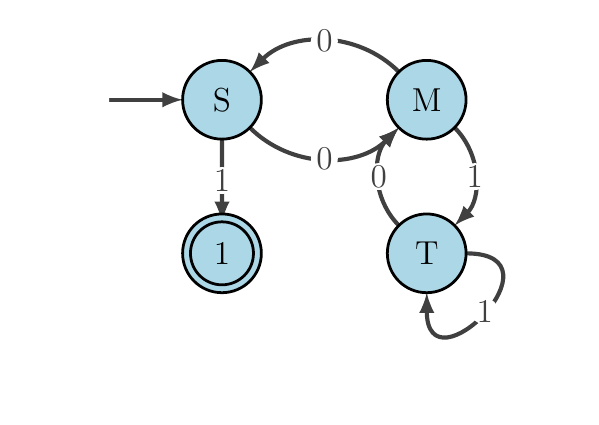
\begin{tikzpicture}[scale=1.3]
				\SetVertexStyle[MinSize=1\DefaultUnit,TextFont=\large]
				\SetEdgeStyle[TextFont=\large]
				\Vertex[x=0,style={color=white}]{Z}
				\Vertex[label=S,x=1.5]{S}
				\Vertex[label=1,x=1.5,y=-1.5]{1}
				\Vertex[label=1,x=1.5,y=-1.5,size=0.8]{1}
				\Vertex[label=M,x=3.5,y=0]{M}
				\Vertex[label=T,x=3.5,y=-1.5]{T}
				\Edge[Direct](Z)(S)
				\Edge[Direct,label=0, bend=-45](S)(M)
				\Edge[Direct,label=1](S)(1)
				\Edge[Direct,label=0,bend=-45](M)(S)
				\Edge[Direct,label=1, bend=45](M)(T)
				\Edge[Direct,label=0, bend=45](T)(M)
				\Edge[Direct,label=1,loopposition=-45,loopshape=90](T)(T)
			\end{tikzpicture}\\
		\subsection{Exercise}
			Write a CFG which describes the parenthesis and addition language
			\begin{align*}
				S\rightarrow :\text{number}:\\
				S\rightarrow :\text{number}:S\\
				S\rightarrow +S\\
				S\rightarrow (S)
			\end{align*}
	\section{uge}
		\subsection{Prove that the best online algorithm for the ski problem has a competitive ratio on $\frac{19}{10}$}
			The ski costed 1 unit to rent a day and 10 to buy.\\
			The online agorithm suggested on buying day 9, which results in a competitive ratio on $\frac{19}{10}$\\
			The alternative is buy on day 5 and day 15\\
			Buy on day 5 worst case scenario is return on day five which cost $14$ for the online algorithm and $5$ if only renting which is a competitive ratio on $\frac{14}{5}$\\
			Buy on day 15 will cost $24$ at worst case and the offline will buy on day 1 which will be $10$ therefore the competitive ratio is $\frac{24}{10}$
		\subsection{For the scheduele algoruthm, what are the result of $m=3$}
			\begin{center}
			\begin{tikzpicture}
				\draw(0,0)rectangle(1.5,1)node[midway]{1};
				\draw(2,0)rectangle(3.5,2)node[midway]{2};
				\draw(4,0)rectangle(5.5,1)node[midway]{1};
				\draw(6,0)rectangle(7.5,4)node[midway]{4};
				\draw(8,0)rectangle(9.5,3)node[midway]{3};
				\draw(10,0)rectangle(11.5,2)node[midway]{2};
			\end{tikzpicture}
			\end{center}
			\begin{tikzpicture}
				\draw(0,0)rectangle(1.5,1)node[midway]{1};
				\draw(2,0)rectangle(3.5,2)node[midway]{2};
				\draw(4,0)rectangle(5.5,1)node[midway]{1};
				\draw(0,1)rectangle(1.5,5)node[midway]{4};
				\draw(4,1)rectangle(5.5,4)node[midway]{3};
				\draw(2,2)rectangle(3.5,4)node[midway]{2};
			\end{tikzpicture}
		\subsection{Make input for any algorithm with $m=2$ which will result in better result than $\frac{3}{2}$ of the optimum}
			From the data 0.3 0.3, if the algorithm stacks 0.3 0.3 we give it the 0.1 input. If it does not stack we give it a 6.
		\subsection{Show that the following data can be in three bins}
			\begin{center}
			\begin{tikzpicture}
				\draw(0,0)rectangle(1.5,0.6)node[midway]{0.2};
				\draw(2,0)rectangle(3.5,1.5)node[midway]{0.5};
				\draw(4,0)rectangle(5.5,1.2)node[midway]{0.4};
				\draw(6,0)rectangle(7.5,2.1)node[midway]{0.7};
				\draw(8,0)rectangle(9.5,0.3)node[midway]{0.1};
				\draw(10,0)rectangle(11.5,0.9)node[midway]{0.3};
				\draw(12,0)rectangle(13.5,2.5)node[midway]{0.8};
			\end{tikzpicture}
			\end{center}
			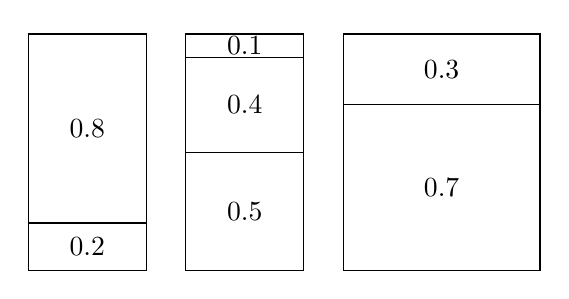
\begin{tikzpicture}
				\draw(0,0)rectangle(1.5,0.6)node[midway]{0.2};
				\draw(2,0)rectangle(3.5,1.5)node[midway]{0.5};
				\draw(2,1.5)rectangle(3.5,2.7)node[midway]{0.4};
				\draw(4,0)rectangle(6.5,2.1)node[midway]{0.7};
				\draw(2,2.7)rectangle(3.5,3)node[midway]{0.1};
				\draw(4,2.1)rectangle(6.5,3)node[midway]{0.3};
				\draw(0,0.6)rectangle(1.5,3)node[midway]{0.8};
			\end{tikzpicture}
		\subsection{Use First Fit on the following data, where the max size is 6}
			\begin{center}
			\begin{tikzpicture}
				\draw(0,0)rectangle(1.5,1)node[midway]{1};
				\draw(2,0)rectangle(3.5,4)node[midway]{4};
				\draw(4,0)rectangle(5.5,3)node[midway]{3};
				\draw(6,0)rectangle(7.5,4)node[midway]{4};
				\draw(8,0)rectangle(9.5,3)node[midway]{3};
				\draw(10,0)rectangle(11.5,1)node[midway]{1};
			\end{tikzpicture}
			\end{center}
			\begin{tikzpicture}
				\draw(0,0)rectangle(1.5,1)node[midway]{1};
				\draw(0,1)rectangle(1.5,5)node[midway]{4};
				\draw(2,0)rectangle(3.5,3)node[midway]{3};
				\draw(4,0)rectangle(5.5,4)node[midway]{4};
				\draw(2,3)rectangle(3.5,6)node[midway]{3};
				\draw(0,5)rectangle(1.5,6)node[midway]{1};
			\end{tikzpicture}
		\subsection{Why can the following result not be amde by First Fit, max size is 9}
			\begin{tikzpicture}
				\draw(0,0)rectangle(1.5,3)node[midway]{3};
				\draw(0,3)rectangle(1.5,8)node[midway]{5};
				\draw(2,0)rectangle(3.5,3)node[midway]{3};
				\draw(4,0)rectangle(5.5,2)node[midway]{2};
				\draw(2,3)rectangle(3.5,7)node[midway]{4};
				\draw(4,2)rectangle(5.5,5)node[midway]{3};
			\end{tikzpicture}
			Because the 2 in the last row would be able to be put on bin 2 and therefore the last bin should only be 3.
		\setcounter{subsection}{0}
		\subsection{Find a squence where $Ff$ performs $\frac{5}{3}$ times worse than OPT}
			$37\cdot (\frac{1}{43}+\frac{1}{10000}),11\cdot (\frac{1}{7}+\frac{1}{10000}),12\cdot (\frac{1}{3}+\frac{1}{10000}),14\cdot(\frac{1}{2}+\frac{1}{10000})$\\
			This will result in bin 1 being filled with $\frac{1}{43}$, then 2 bins with $\frac{1}{7}$, then 6 bins with 2 thirds and 13 bins with a half. In total 22\\
			For OPT it will make 11 bins with 1 half, 1 third, $\frac{1}{7}$ and $\frac{1}{43}$ and two bins with the rest. Therefore the result is $\frac{22}{13}$
	\section{Uge}
		\subsection{Which of the following formulas are satisfiable}	
			\subsubsection{$A\land B$}
				Satisfiable if $A$ and $B$ are true	
			\subsubsection{$A\lor B$}
				Satisfiable if $A$ or $B$ are true
			\subsubsection{$A\rightarrow B$}
				Satisfiable if $A$ and $B$ are true
			\subsubsection{$A\land \neq A$}
				Not satisfiable 
			\subsubsection{$A\lor \neg A$}
				Satisfiable always true
		\subsection{Which if the following formulas are equivalent (same assignment satisfy)}
			\begin{enumerate}
				\item $\neg A\land B$
				\item $\neg A\lor B$
				\item $A\rightarrow B$
				\item $(A\rightarrow B)\land (\neg B\rightarrow A)$
				\item $(\neg A\rightarrow B)\land (\neg B\rightarrow \neg A)$
			\end{enumerate}
				For these the same assignment will return true\\
				1=2=3=5\\
				4=2=3=5\\
				But 2 and 3 are equivalent and 4 and 5 are equivalent
		\subsection{Convert the following formulas into CNF}
			\subsubsection{$\neg A\land B$}
			\subsubsection{$\neg A\lor B$}
			\subsubsection{$A\rightarrow B$}
				$\neg A \lor B$
			\subsubsection{$(A\rightarrow B)\land(\neg B\rightarrow A)$}
				$(\neg A \lor B)\land (B\lor A)$\\
		\subsection{Breaking symmetry in N-Towers and N-Queens}
			\subsubsection{Write two clauses that forbid solutions where there is a queen in the irght half of the first row}
				$(\neg X_{1,1})\land (\neg X_{1,2})$
			\subsubsection{Instead of adding two clauses change an existing clause}
				$(X_{1,1}\lor X_{1,2}\lor X_{1,3} \lor X_{1,4})$ to $(X_{1,3}\lor X_{1,4})$
				This will determine that it must be either one of those two.
		\setcounter{subsection}{5}
		\subsection{The formula from Slide 11 contains redundant information. FOr Example $X_{1,1}\rightarrow\neg X_{1,2}$ and $X_{1,2}\rightarrow \neg X_{1,1}$ are equivalent. Understand and remove these redundancies:}
			\subsubsection{Why do these redundancies occur?}
				They are often not directly identifliable since to construct a boolean formula it is often taken from one end to another.
			\subsubsection{Identify all such redundacies!}
				\begin{align*}
					X_{1,1}\rightarrow \neg X_{1,2}\equiv X_{1,2}\rightarrow \neg X_{1,1}\\
					X_{1,1}\rightarrow \neg X_{2,1} \equiv X_{2,1}\rightarrow \neg X_{1,1}\\
					X_{1,2}\rightarrow \neg X_{2,2} \equiv X_{2,2}\rightarrow \neg X_{1,2}\\
					X_{2,1}\rightarrow \neg X_{2,2}\equiv X_{2,2}\rightarrow \neg X_{2,1}
				\end{align*}
			\subsubsection{Write down a simplified formula without redundancies}
				It the right row of the previus align plus $X_{1,1}\lor X_{1,2}\land X_{2,1}\lor X_{2,2}$
			\subsubsection{Convert the formula to CNF}
			$[[\neg X_{1,1}\neg X_{1,2}],[ \neg X_{1,1}, \neg X_{2,1} ],[ \neg X_{1,2}, \neg X_{2,2}],[\neg X_{2,1}, \neg X_{2,2}],[ X_{1,1}, X_{1,2}],[ X_{2,1}, X_{2,2}]]$
			\subsubsection{Write the formula in DIMACS format}
				p cnf 4 6\\
				-1 -2 0\\
				-1 -3 0\\
				-2 -4 0\\
				-3 -4 0\\
				1 2 0\\
				3 4 0
			\subsubsection{Run it in a SAT and test result}
			Result - $v 1 -2 -3 4 0$\\
			It here came up with a result with the tower in upper left and lower right
		\setcounter{subsection}{0}
		\subsection{Which of the following formulas are satisfiable}
			\subsubsection{$(A\rightarrow B) \land (B\rightarrow A)$}
				$A$ and $B$ true
			\subsubsection{$(A\rightarrow B) \land (B\rightarrow A)\land A$}
				$A$ and $B$ true
			\subsubsection{$(A\rightarrow B) \land (B\rightarrow A)\land \neg A$}
				$A$ and $B$ false
			\subsubsection{$(A\rightarrow B) \land (B\rightarrow A)\land (\neg A\rightarrow \neg B)\land (\neg B\rightarrow A)$}
				$A$ and $B$ true
		\subsection{Whuch of the following formulas are equivalent}
			\begin{itemize}
				\item $(A\rightarrow B)\land (\neg B \rightarrow A)$
				\item $(A\rightarrow \neg B)\land B\rightarrow A)$
				\item $(\neg A\lor \neg B)\land (A\lor\neg B)$
				\item $(B\lor A)\land (\neg A \lor B)$
			\end{itemize}
			$A$ and $B$ true\\
			1,4\\
			$A$ true, $B$ false\\
			2,3\\
		\subsection{Convert to CNF}
			\subsubsection{$(\neg A\rightarrow B)\land (\neg B\rightarrow \neg A)$}
				$(A\lor B)\land (B\lor \neg A)$
			\subsubsection{$A\rightarrow (\neg(B\land D))$}
				$\neg A\lor \neg B\lor \neg D$
			\subsubsection{$A\rightarrow(\neg(B\lor D))$}
				$\neg A\lor (\neg B \land \neg D)$
			\subsubsection{$A\rightarrow (\neg(B\rightarrow(C\land D)))$}
				$\neg A \lor B \land \neg C\lor \neg D$
	\section{47}
		\subsection{Given the follwing relation schema:}
			$$Band(name: CHAR(20), formed_in: INTEGER)$$
			Whihc of the following are valid tuples of the Band relation?\\
			\begin{itemize}
				\item ('Foo Fighters',1994)
				\item (1991, 'Incubus')
				\item ('Massive Attack')
				\item ('Disturbed, '1996')
			\end{itemize}
			1\\
		\clearpage
		\subsection{The relation schema of task 1 together with the vald tuples define a relation instance. Visualize this relation instance as a table}
			\begin{table}[]
				\begin{tabular}{|l|l|}
				\hline
				Band         & formed\_in \\ \hline
				Foo fighters & 1994       \\ \hline
				\end{tabular}
			\end{table}
		\subsection{Given the following relation instance}
			\begin{figure}[h!]
				\centering
				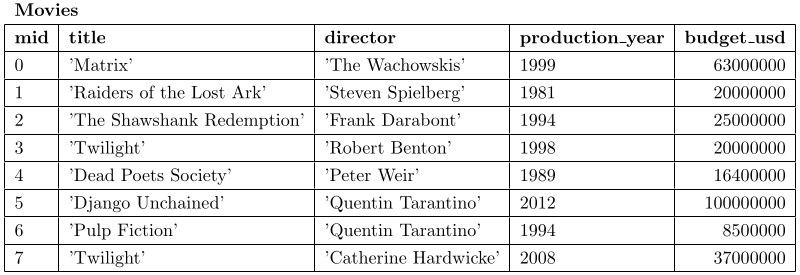
\includegraphics[width=250px]{images/47,2.png}
				\label{}
				\caption{}
			\end{figure}
			Which of the following atributes sets are possible primary keys (i.e., the data instance above is consistent with choosing that set of attributes as the primary key)?
			\begin{itemize}
				\item {mid}
				\item {title}
				\item {director}
				\item {title, director}
				\item {director, production\_year}
			\end{itemize}
			1, 4, 5
		\subsection{Given the following Entity-Relationship diagram}
			\begin{figure}[h!]
				\centering
				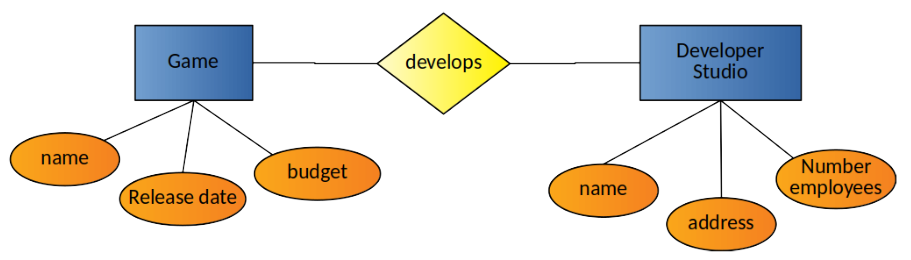
\includegraphics[width=250px]{images/47,3.png}
				\label{}
				\caption{}
			\end{figure}
			How could this ER diagram be modeled in the relational model? Provide the relation schemas. What would change if the relationship "develops" had an attribute "start date"? Note that here is no desingation of keys for entities. It is part of the task to consider what is a good choice of keys (this is a data modeling choice, for which there is no single "right answer")	
			GAME('name':char(20),'Release date': char(10), 'Budget': integer)\\
			Developer Studio('name': char(20),'Address':char(40),'Number employees':integer)\\
			develops('name':char(20),'address': char(40))\\
		\subsection{You are given the relation instance defined in task 3}
		How many tuples do the relations resulting from the following relational operations contain? [Recall that in the relational mode, relations are sets, so there cna be no duplicates among (entire) tuples/rows.]
		\begin{itemize}
			\item $\sigma_{prodution_year>1994}(Movies)$ - 4
			\item $\pi_{mid,title,director}(Movies)$ - 8
			\item $\pi_{director}(Movies)$ - 7
		\end{itemize}
		\subsection{You are given the following ER-diagram:}
			\begin{figure}[h!]
				\centering
				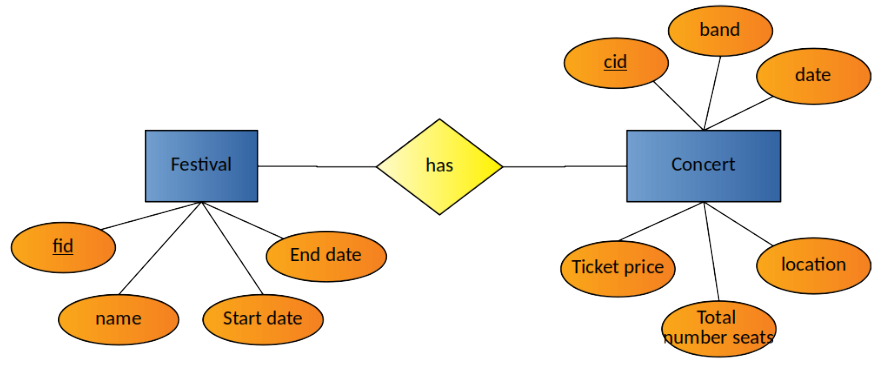
\includegraphics[width=250px]{images/47,6.png}
				\label{}
				\caption{}
			\end{figure}
			and the corresponding relations:\\
			\begin{itemize}
				\item Concert(cid: integer, band: char(20),date char(20), locaton: char(20), tital\_number\_seats: integer, ticket\_price: float)
				\item Festival(fid integer, name: char(20), start\_date: char(20), end\_date: char(20))
				\item FestivalHasConcert(festival: integer, concert: integer)
			\end{itemize}
			Here, underlined attributes are primary keys of the relation and dashed
			underlined attributes are foreign keys.
			Specify the SQL command that creates the table corresponding to the
			Concert relation of task.
			Also specify the SQL command that creates a corresponding table for
			the FestivalHasConcert relation.
			[Recall that FestivalHasConcert’s festival and concert attributes are
			foreign keys referencing the fid in the festival and cid in the concert relation]	\\[4mm]
			CREATE table Concert(cid: integer, band: char(20), date: char(20),location: char(20), total\_number\_sears: integer, ticker\_price: float, Primary Key (cid))\\
			CREATE table FestivalHasConcert(festival: integer foreign key reference Concert(cid), concert integer foreign key reference Festival(fid))\\
			May also be FOREING KEY (concert) REFERENCES Concert
		\subsection{Specify an SQL command that deletes formthe Moveis table all moeis that were not produced in 1994}
			DELETE FROM Moveis WHERE production\_year != 1994;
		\subsection{You want to retrive the titles f all moveis from the Moviestable of task3 that were produced in 1994 and directed by Quentin Tarantino. Express the query in bth theese ways:}
			\begin{itemize}
				\item As an expression in relational algebra
				\item As an SQL command
			\end{itemize}
				$\pi_{title}\sigma_{prouction\_year = 1994 \land director =  "Quentin Tarantino"}(Movies)$\\
				Select title From Movies where production\_year == 1994 and director == "Quentin Tarantino"
		\subsection{Consider the Movies table of task 3. Provide in SQL one INSERT and one DELETE command that can to be executed to change it into the following table}
			\begin{figure}[h!]
				\centering
				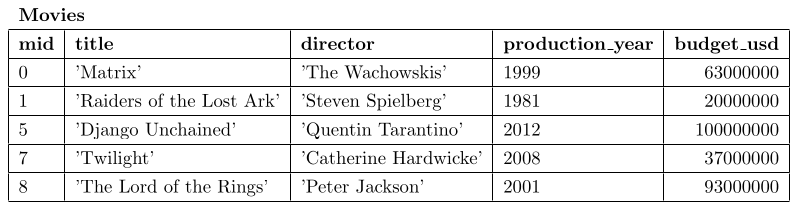
\includegraphics[width=250px]{images/47,10.png}
				\label{}
				\caption{}
			\end{figure}
			DELTE FROM Movies WHERE production\_year $<$ 1995 and production\_year $>$ 1988\\
			INSERT INTO Movies (9,'The Lord of the Rings', 'Peter Jackson', 2001, 93000000)
		\subsection{Specify an SQL command withot set operations (UNION or EXCEPT) that retirves all movies from the Movie table, that have been produced before 1990 or that have a budget of at least 30 million USD. State the same query as an relational algebra expression}
			SELECT * FROM Movies WHERE production\_year $<$ 1990 or 30000000 $<$ budget\_usd\\
			$\sigma_{production\_year < 1990 \lor 30000000 < budget\_usd}(Movies)$
		\subsection{Solve task 10 with SQL operations (UNION OR EXCEPT). State the same query as an relational algebra expression.}
			SELECT * FROM Movies WHERE production\_year $<$ 1990 EXCEPT SELECT * FROM Movies Where budget\_usd $>$ 30000000\\
			$\sigma_{production\_year < 1990} - \sigma_{budget > 30000000}$
		\subsection{Specify an SQL command without set operations (UNION or EXCEPT) that retrieves all movies from the Movie table if task 3 that either}
		\begin{itemize}
			\item have been produced before 100- with a bduget of at least 30 million USD
			\item or have been produced after 2010
		\end{itemize}
		SELECT * FROM Movies WHERE production\_year $<$ 1990 and budget\_usd $>$ 30000000 or 2010 $<$ production\_year \\
		\subsection{Specify an SQL command that retireves all pairs of movies from the Movies table fo task 3 that have been directed by the same director.}
		For instance if two movies 'movie1\ and 'movie2' were directed by te same director, the result relation should, amongst others, contain the followingt tuples:
		\begin{itemize}
			\item (movie1, movie2)
			\item (movie2, movie1)
		\end{itemize}
		SELECT title FROM Movies WHERE director as dir CROSS JOIN SELECT title FROM Movies WHERE director = c \\
		ALTERNATIVE\\
		SELECT * FROM Movies M1, Movies M2 WHERE M1.director = M2.director AND M1.mid != M2.mid
		\subsection{SPecify an SQL command that retrieves all pairs of mvoes (move1, movie2) from the Movies table fo task 3 with movie1's budget exceeding the budget if movie2}
			For instance if a movie 'movie5' has a larger budget than 'movie8', the result relation should contain, amongst others the following tuple: (movie5,movie8)\\
			State the same query as an relational algebra expression\\
		SELECT title FROM Movies WHERE budget as bud CROSS JOIN SELECT title FROM Movies WHERE budget $<$ bud\\
		Alt. SELECT $*$ FROM Movies M1, Movies M2 WHERE M1.budget\_uds $>$ M2.budget\_usd;
	\setcounter{subsection}{0}
	\subsection{Which of the following statements are true?}
		\begin{itemize}
			\item \checkmark The result of applying a relational algebra operator to a relation instance is another relation instance
			\item Entities of the ER-diagram can not be described by relations in the data model.
			\item A relation instance needs to contain at least one tuple
			\item Integrity coonstraintss are specified when querying the databae
			\item \checkmark Primary keys and foreign keys are types of integrity constraints
			\item The relational selection operator always returns a relation instance with fewer tuples.
			\item \checkmark The relational projection operator may return a relation instance with fewer tuples.
			\item The SQL UNION operator can be applied to two relation instances if they have the same number of attributes
		\end{itemize}
	\subsection{Joins are compound operator which we did not cover in the lcture. They are useful for joining (combining) the data contained in muliple relations together. In relaional algebra the conditional join operator $\bowtie_C$ (also called the $\theta$-join operator) is defined by}
		$$R1\bowtie R2=\sigma_C (R_1\times R_2)$$
	In words: A conditional join can be calculated by first computing the cross product of the two relations $R1$ and $R2$ followed by a selection using the condition $C$.\\
	We now look at the following condiition join on relatiosn from task 6.\\
	Festival $\bowtie_{fid=festival}$ FestivalHasConcert\\
	This join combines the two relations Festival and FestivalHasConcert using the attribute fid of the Festival relation, and the festival attribute of the FestivalHasConcert relation. SPecifically it combines those tuples of the two relations for which the equality condition holds.\\
	What is the relation schema of the result relation?\\
	It returns a tuples with the festival and concert id if the concert is at the festival.
	\subsection{Specify an SQL command that calculates hte conditional join given in task 2}
	SELECT name, cid FROM Festival, FestivalHasConcert WHERE Festival.fid = FestivalHasConcert.fid
	\subsection{Specify an SQL command that calculates the following nested relational operation involving two conditional joins}
	Festival$\bowtie_{fid=festival}$FestivalHasConcert$\bowtie_{concert=cid}$Concert\\
	SELECT cid, fid FROM Festival,FestivalHasConcert,Concert WHERE Festival.fid = FestivalHasConcert.fid and FestivalHasConcert.cid = Concert.cid;
\section{Uge}
	THe following answers a gathered through the RSA program.
	\subsection{Suppose in RSA the public key is $PK=(1517,13)$. Which of the following is the RSA encryption if the message $43$}
		$E(m,PK)=894$ mod $1517$\\
		$43^{13} $ (mod 1517) $=894$ mod 1517\\
	\subsection{Is one of the following the multiplicative inverse if 49 modulo 221}
		$212$
	\subsection{Which of the following sets of public key (OK) and secret key (SK) is a valid set of RSA keys (igoring the numbers are not large eneough)}
		\subsubsection{$PK=(91,37);SK=(91,23)$}
			$91=7\cdot 13$\\
			$37\cdot 23\equiv 1$ (mod$(7-1)\cdot (13-1)$)\\
			$851\equiv 1$ (mod 72)\\
			$851\equiv 59$ (mod 72)\\
			Not a working pair
		\subsubsection{$PK=(143,77);SK=(143,53)$}
			$143=11\cdot 13$\\
			$77\cdot 53\equiv 1$ (mod$(11-1)\cdot (13-1)$)
			$4081\equiv 1$ (mod 120)\\
			This works!
		\subsubsection{$PK=(231,59);SK=(231,47)$}
			$231$ has a prime facotrization of 3,7 and 11 and therefore not a valid number
		\subsubsection{$PK=(107,25);SK=(107,30)$}
			$107$ is a prime and therefore not valid
	\subsection{In the Sieve of Eratosthemes, how many lists have been created at the point where the number 13 is the first elment in the list?}
			The first elements will be:\\
			$2,3,5,7,11,13$
			Therefore 6
	\subsection{Consider an RSA system with ALice public key $n=1517$ and $e=17$. Note that $1517=37\cdot 41$.}
		\subsubsection{Find Alices secret key $d$. Use the extended Euclidean Algorithm from page 42 of the slies from the lecture}
			$(37-1)\cdot(41-1)=1440$\\
			$gcd(17,1440)=1$\\
			$17\cdot 593\%1440=1$\\
			$d_a=593$
		\subsubsection{Try encrypting 423. Use the algorithm for fast modular exponentiation. How many times during the recursive execution is the $if$ $k$ is odd case encountered?}
			5
		\subsubsection{Decrypt the number obtained above, how many times odd and even?}
			Worked, 17 even 5 odd
	\subsection{Why is cryptopographically secure hash function used in connection with RSA digital signatures?}
		It is a wasy to secure a signature and will make it harder to forge due to not only needing to crack the key but also have to make the hash correct too.
	\subsection{With RSA why would you never use the valeu 2 as one of the two primes $p$ and $q$}
		Due to it would be very easy to bruteforce the other prime.
	\subsection{In RSA why must the message being encrypted be a non negative integer strictly less than the modulos}
		Otherwise the data will be lost.
	\setcounter{subsection}{0}
	\subsection{Try breaking these two encrypted messages}
		\subsubsection{Caesar cipher in english}
			YMNX HWDUYTLWFR NX JFXD YT IJHNUMJW.\\
			THIS CRXPTOGRZM IS EZSX TO DECIPHERB - shift 20
		\subsubsection{Decrypt mono-alphabetic cipher}
			TOWWJPHJC ZY RXW PHOTWYR ZYPHJC ZJ RXW SFOPC. UFYR FB ZR ZY QFIWOWC SZRX ZQW RXFMYHJCY FB BWWR CWWD.\\
			GREENLAND IS THE LARGEST ISLAND IN THE WORLD. MOST OF IT IS COVERED WITH ICE THOUSANDS OF FEET DEEP.
\section{Uge}
	\subsection{Why in RSA is it necessary that $gcd(e_A,(p_A-1)(q_A-1))=1$?}
		Because otherwise it would not be able to get the information back due to some values will not result in the message comming back
	\subsection{Draw the graph reprensenting the road system in the figure below, and write down the number of verties, the number of edges and the degree of each vertex}
	$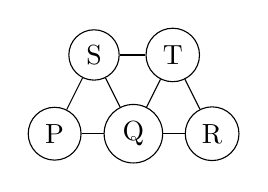
\begin{tikzpicture}[scale=1]
				\tikzstyle{vertex}=[circle,draw=black]
				\node[vertex](v1) at (0,0){P};
				\node[vertex](v2) at (1,0){Q};
				\node[vertex](v3) at (2,0){R};
				\node[vertex](v4) at (0.5,1){S};
				\node[vertex](v5) at (1.5,1){T};
				\path[-]
					(v1) edge node {}(v2)
					(v1) edge node {}(v4)
					(v2) edge node {}(v3)
					(v2) edge node {}(v4)
					(v2) edge node {}(v5)
					(v4) edge node {}(v5)
					(v5) edge node {}(v3);
			\end{tikzpicture}$
	\subsection{On Twitter:}
		\subsubsection{John follows Joan, Jean and Jane; Joe follows Jane and Joan; Jean and Joan follow each other. Draw a diagraph illustrating these follow relationships between John, Joan, Jane and Joe.}
		$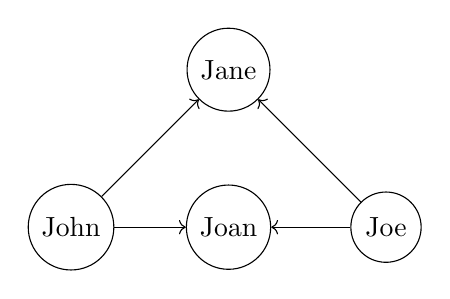
\begin{tikzpicture}[scale=2]
			\tikzstyle{vertex}=[circle,draw=black]
				\node[vertex](v1) at (0,0){John};
				\node[vertex](v2) at (1,0){Joan};
				\node[vertex](v3) at (2,0){Joe};
				\node[vertex](v4) at (1,1){Jane};
				\path[->]
					(v1) edge node {}(v4)
					(v1) edge node {}(v2)
					(v3) edge node {}(v2)
					(v3) edge node {}(v4);
			\end{tikzpicture}$
		\subsubsection{Twiter has 313 million active users (June 2016, based on Twitter Inc.) Imaging you would like to store the diagraph for the follow relationships in an adjecency matrix that uses 4 bytes per entry on your new laptop which has 64 gb of RAM. Is this feasible}
			\begin{align*}
				313000000\cdot 313000000\\
				\text{Entries:}\;97969\cdot 10^{12}\\
				97969\cdot 10^{12}\cdot 4\\
				3.91876\cdot 10^{17}\;\text{Bytes}\\
				3.91876\cdot 10^{17}\cdot 0.0000000009\\
				36\cdot 10^6\;\text{gb}
			\end{align*}
			It would use 36 million gb of data
		\subsubsection{The municipality of Odense has a population of 200000 people. Let $G$ be the graph where the meaning of an edge from vertex $i$ to $j$ is "person $i$ is friends with person $j$". Imagine you would like to store the adjacency matrix for this graph for the relationships in a matrix representation that ises 4 bytes per entry on your new lapto which has 64 GB of RAM. Is this feasible?}
			\begin{align*}
				200000\cdot 200000\\
				40\cdot 10^9\;\text{entries}\\
				120\cdot 10^9\;\text{bytes}\\
				120\cdot 10^9\cdot 0.0000000009\\
				108
			\end{align*}
			It would use 108 gb of ram
		\subsection{Consider the following six graphs (note tat the nodes do not have labels).}
			\begin{figure}[h!]
				\centering
				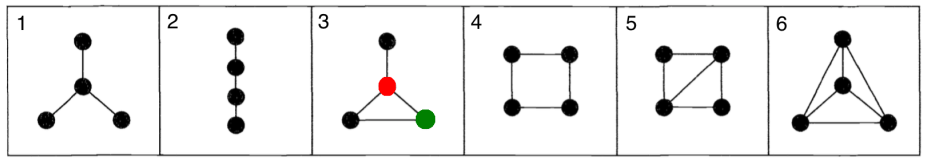
\includegraphics[width=250px]{images/49,5.png}
				\label{}
				\caption{}
			\end{figure}
			
			\subsubsection{How many walks of length 3 formthe red vertex to the green vvertex are there in graph 3?}
				4
			\subsubsection{How many paths from the red vertex to the green vertex are there in graph 3}
				2
			\subsubsection{How many shortest paths from the red vertex to the green vertex are there in graph 3?}
				1
			\subsubsection{For each of the graphs: what is the longest of all pairwise shortest paths?}
				\begin{itemize}
					\item 2
					\item 3
					\item 3
					\item 4
					\item 5
					\item 5
				\end{itemize}
			\subsubsection{Give an adjancency matrix for graph 1. Can there be different adjaccency matrices for the same graph? If so name a second adjacency matrix for graph 1. Can you find two different adjacency matrices for graph 6?}
				$\begin{bmatrix}
					0&1&0&0\\
					1&0&1&1\\
					0&1&0&0\\
					0&1&0&0
				\end{bmatrix}$
				Its possibble to move the second row up and down.
				The same argument goes for number 6
		\subsection{Let $A$ be an adjacency matrix. In the lecture you learned that the $ij$-entry of $A^k$ is the number of different walks from vertex $i$ to vertex $j$ using exactly $k$ edges}
			\subsubsection{What is the interpretation of $ij$-entry of the matrix $A^1+A^2+A^3$?}
				If a walk exists with all 3 lengths it would be 6 otherwise i can be lower if a path does not exists in the given length.
			\subsubsection{Complete the following sentence with the missing expression: In a graph $G$ with adjacency matrix $A$, vertex $i$ and $j$ are connected if and only if $...>0$.}
				$ij$ entry has a value
		\setcounter{subsection}{0}
		\subsection{Find four different square roots of 1 modulo 143, i.e., numbers which multiplied by themselves modulo 143 give 1 (and which are at least 0 and less than 143). You may consider writing a simple program for finding them.}
			12, 131, 142, 144
		\subsection{Try executing the Miller-Rabin primality test on 11, 15, and 561.}
			\subsubsection{What types of numbers are they?}
				11 is prime\\
				15 is composite\\
				561 is carmichael number
			\subsubsection{Which numbers showed it was a composit?}
				15 was showed by 9\\
				561 was showed by 35
	\section{Uge}
		\subsection{Let the following weighted graph G (from the lecture slides, weights are depicted in red) be given:}
			\begin{minipage}{0.45\textwidth}
			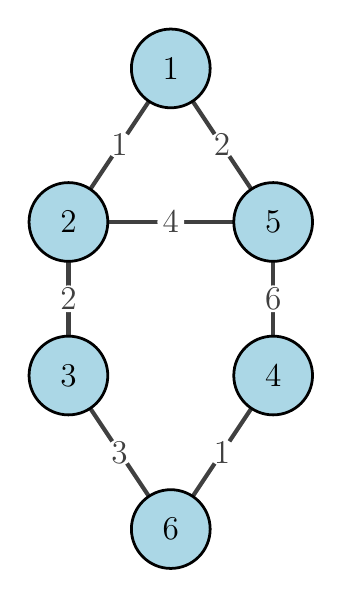
\begin{tikzpicture}[scale=1.3]
				\SetVertexStyle[MinSize=1\DefaultUnit,TextFont=\large]
				\SetEdgeStyle[TextFont=\large]
				\Vertex[label=1,x=1]{A}
				\Vertex[label=2,x=0,y=-1.5]{B}
				\Vertex[label=5,x=2,y=-1.5]{C}
				\Vertex[label=3,x=0,y=-3]{D}
				\Vertex[label=4,x=2,y=-3]{E}
				\Vertex[label=6,x=1,y=-4.5]{F}
				\Edge[label=1](A)(B)
				\Edge[label=2](A)(C)
				\Edge[label=4](B)(C)
				\Edge[label=2](B)(D)
				\Edge[label=6](C)(E)
				\Edge[label=3](D)(F)
				\Edge[label=1](E)(F)
			\end{tikzpicture}\\
		\end{minipage}
		\hfill
		\begin{minipage}{0.45\textwidth}
			D=\bordermatrix{ &1 & 2 & 3 & 4 & 5 & 6 \cr
			      1 & 0 & 1 & 3 & 7 & 2 & 6 \cr
			      2 & 1 & 0 & 2 & 6 & 3 & 5 \cr
			      3 & 3 & 2 & 0 & 4 & 5 & 3 \cr
			      4 & 7 & 6 & 4 & 0 & 6 & 1 \cr
			      5 & 2 & 3 & 5 & 6 & 0 & 7 \cr
			      6 & 6 & 5 & 3 & 1 & 7 & 0
}
		\end{minipage}
		\subsubsection{How many shortest path in $G$ are of length 6? Name them.}
			1 - 6\\
			4 - 5\\
			2 - 4
		\subsubsection{How long is the longest of all pairwise shortest paths in the graph? Are there several longest shortest paths?}
			7 \\
			1 - 4\\
			5 - 6
		\subsubsection{How many paths in $G$ are of length 6? (Note: a path does not necessarily need to be a shortest path.) Name them.}
			18 because there exists path from every point to another with the length of 6
	\subsection{Assume in this exercise that all weights on edges are non-negative values.}
		\subsubsection{In a graph $G$ with $n=6$ vertices, how man matrix-matrix multiplication operations are needed in the worst case in order to compute the distance matrix $D$, when the method of repeated squaring is used to compute $D$}
			$\log_2(6-1)= 1.61$ - so two operations
		\subsubsection{In a graph $G$ with $n=200$ vertices, how many matrix-matrix multiplications are needed in the worst case in order to compute the distance matrix $D$, when the method of repeated squaring is used to compute $D$?}
			$\log_2(199)= 5.3$ - so 6 operations		
		\subsubsection{Can yopu find a graph $G$ with $n=6$ vertices for which $W^4\neq W^5$? if so depict it}
			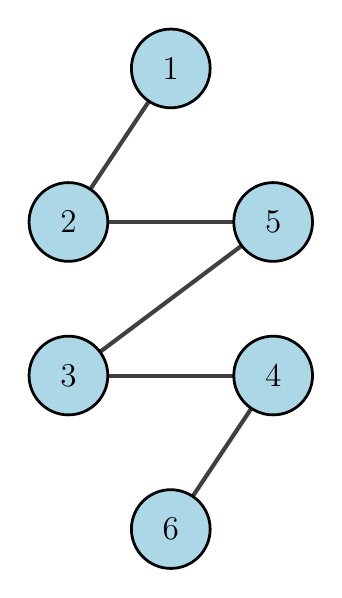
\begin{tikzpicture}[scale=1.3]
				\SetVertexStyle[MinSize=1\DefaultUnit,TextFont=\large]
				\SetEdgeStyle[TextFont=\large]
				\Vertex[label=1,x=1]{A}
				\Vertex[label=2,x=0,y=-1.5]{B}
				\Vertex[label=5,x=2,y=-1.5]{C}
				\Vertex[label=3,x=0,y=-3]{D}
				\Vertex[label=4,x=2,y=-3]{E}
				\Vertex[label=6,x=1,y=-4.5]{F}
				\Edge[](A)(B)
				\Edge[](B)(C)
				\Edge[](C)(D)
				\Edge[](D)(E)
				\Edge[](E)(F)
			\end{tikzpicture}\\
			
		\subsubsection{Can yopu find a graph $G$ wit h$n=6$ vertices for which $W^5 \neq W^6$? if so depict it}
			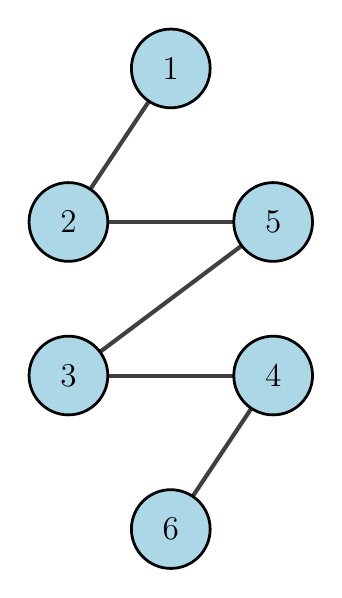
\begin{tikzpicture}[scale=1.3]
				\SetVertexStyle[MinSize=1\DefaultUnit,TextFont=\large]
				\SetEdgeStyle[TextFont=\large]
				\Vertex[label=1,x=1]{A}
				\Vertex[label=2,x=0,y=-1.5]{B}
				\Vertex[label=5,x=2,y=-1.5]{C}
				\Vertex[label=3,x=0,y=-3]{D}
				\Vertex[label=4,x=2,y=-3]{E}
				\Vertex[label=6,x=1,y=-4.5]{F}
				\Edge[](A)(B)
				\Edge[](B)(C)
				\Edge[](C)(D)
				\Edge[](D)(E)
				\Edge[](E)(F)
			\end{tikzpicture}\\
		\subsubsection{Can yopu find a graph $G$ wit h$n=6$ vertices for which $W^1= W^2$? if so depict it}
			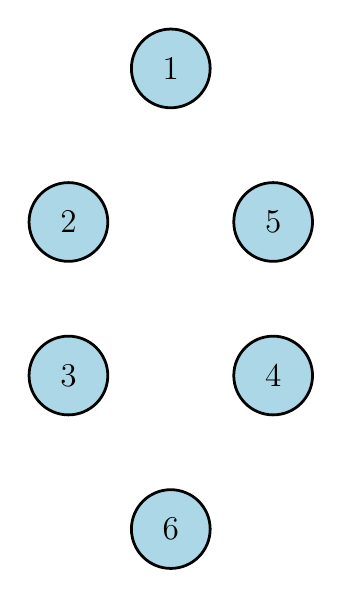
\begin{tikzpicture}[scale=1.3]
				\SetVertexStyle[MinSize=1\DefaultUnit,TextFont=\large]
				\SetEdgeStyle[TextFont=\large]
				\Vertex[label=1,x=1]{A}
				\Vertex[label=2,x=0,y=-1.5]{B}
				\Vertex[label=5,x=2,y=-1.5]{C}
				\Vertex[label=3,x=0,y=-3]{D}
				\Vertex[label=4,x=2,y=-3]{E}
				\Vertex[label=6,x=1,y=-4.5]{F}
			\end{tikzpicture}\\
		\subsubsection{What is the computational runtime in order to compute the distance matrix $D$ for a graph $G$ with $n$ vertices if the method of repeated squaring is used to compute $D$?}
			$O(\log_2{n-1})$
	\subsection{Consider the following molecule (it’s called 2,3-Dimethylhexane}
			\begin{figure}[h!]
				\centering
				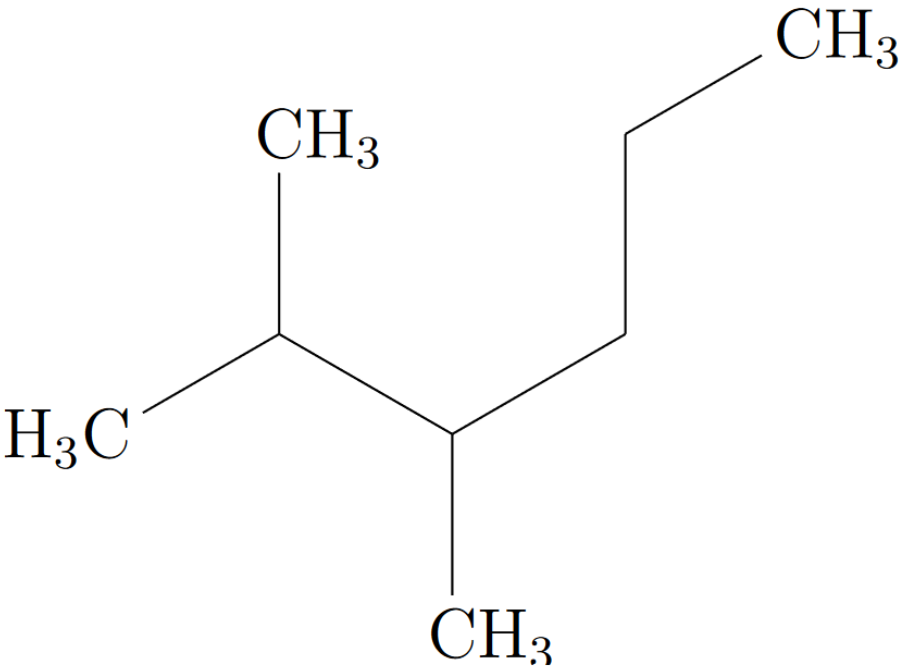
\includegraphics[width=150px]{images/50,3.png}
				\label{}
				\caption{}
			\end{figure}
		\subsubsection{How many carbon atoms does this molecule have?}
			8 carbons
		\subsubsection{Draw the graph $G$ corresponding to the carbon backbone of the molecule}
			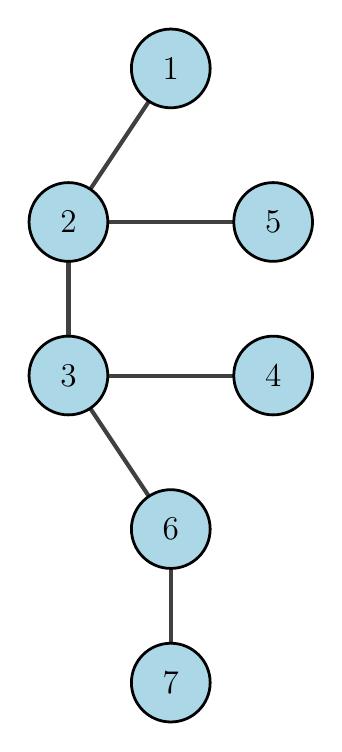
\begin{tikzpicture}[scale=1.3]
				\SetVertexStyle[MinSize=1\DefaultUnit,TextFont=\large]
				\SetEdgeStyle[TextFont=\large]
				\Vertex[label=1,x=1]{A}
				\Vertex[label=2,x=0,y=-1.5]{B}
				\Vertex[label=5,x=2,y=-1.5]{C}
				\Vertex[label=3,x=0,y=-3]{D}
				\Vertex[label=4,x=2,y=-3]{E}
				\Vertex[label=6,x=1,y=-4.5]{F}
				\Vertex[label=7,x=1,y=-6]{G}
				\Edge[](A)(B)
				\Edge[](B)(C)
				\Edge[](B)(D)
				\Edge[](D)(E)
				\Edge[](D)(F)
				\Edge[](F)(G)
			\end{tikzpicture}\\
			
		\subsubsection{Give the edge weight matrix $W$ for the graph $G$}
			W=\bordermatrix{ &1 & 2 & 3 & 4 & 5 & 6 & 7 \cr
			      1 & \infty & 1 & \infty & \infty & \infty & \infty & \infty \cr
			      2 & 1 & \infty & 1 & \infty & 1 & \infty &\infty \cr
			      3 & \infty & 1 & \infty & 1 & \infty & \infty & \infty \cr
			      4 & \infty & \infty & 1 & \infty & \infty & \infty & \infty \cr
			      5 & \infty & 1 & \infty & \infty & \infty & \infty & \infty \cr
			      6 & \infty & \infty & 1 & \infty & \infty & \infty & 1 \cr
			      7 & \infty & \infty & \infty & \infty & \infty & 1 & \infty
}
		\subsubsection{Use your brain or the Java program ShortestPaths.java to infer the distance matrix. }
	W=\bordermatrix{ &1 & 2 & 3 & 4 & 5 & 6 & 7 \cr
			      1 & 2 & 1 & 2 & 3 & 2 & 3 & 4 \cr
			      2 & 1 & 2 & 1 & 2 & 1 & 2 &3\cr
			      3 & 2 & 1 & 2 & 1 & 2 & 1 & 2\cr
			      4 & 3 & 2 & 1 & 2 & 3 & 2 & 3\cr
			      5 & 2 & 1 & 2 & 3 & 2 & 3 & 4\cr
			      6 & 3 & 2 & 1 & 2 & 3 & 2 & 1 \cr
			      7 & 4 & 3 & 2 & 3 & 4 & 1 & 2
}
		\subsubsection{What is the Wiener Index $W(G)$}
			$W(G)= 0.5\cdot 106=58$
		\subsubsection{How many shortest paths of length $3 i \rightarrow ...\rightarrow j$ with $i<j$ are in $G$}
			6
		\subsubsection{Using Wiener’s method for predicting the boiling point, what is your prediction for 2,3-Dimethylhexane?}
			\begin{align*}
				n= 8\\
				t_0=745.42\cdot\log_{10}(n+4.4)-689.4=125.66\\
				w_0=\frac{1}{6}\cdot(n+1)\cdot n \cdot (n-1) = 84\\
				p_0=n-3=5\\
				p=6\\
				t_B=t_0-(\frac{98}{n^2}(w_0-W(G))+5.5\cdot(p_0-p)=96.85
			\end{align*}
	\subsection{Assume in this exercise that all weights on edges are non-negative values. Prove the following theorem stated on the slides}
		If $G$ is a weighted graph with edge weight matrix $W$, and vertices with indices $1,...,n$ then for each positive interger $k$ the $ij$-th entry of\\
		$$W^k=W\odot W\odot ... \odot W$$ - k times\\
		is the length of the shortest path from $i$ to $j$ using maximally $k$ edges. Prove this theorem by induction over $k$\\
		For a graph with two connected vertices, be multiplying the matrix, it will only contain a number larger than 0 if there is at least two edge connected to the vertice. If more is connected it will create a number equal to the number of path with the given length.
		
		

			

		



\end{document}


